\documentclass[11pt]{article}
\usepackage[margin=0.82in]{geometry}
\usepackage[T1]{fontenc}
\usepackage[utf8]{inputenc}
\usepackage{lmodern}
\usepackage{amsmath,amssymb}
\usepackage{graphicx}
\usepackage{booktabs}
\usepackage{tabularx}
\usepackage{array}
\usepackage{pdflscape}
\usepackage{float}
\usepackage{xcolor}
\usepackage{microtype}
\usepackage{hyperref}
\hypersetup{colorlinks=true,linkcolor=blue!55!black,urlcolor=blue!55!black,citecolor=blue!55!black}
\setlength{\parindent}{0pt}
\setlength{\parskip}{0.55em}

\newcounter{suppalgorithm}
\newenvironment{suppalgorithm}[1]{%
  \refstepcounter{suppalgorithm}%
  \par\medskip\noindent\hrule\smallskip
  \noindent\textbf{Algorithm \thesuppalgorithm. #1}\par\smallskip
}{%
  \par\smallskip\noindent\hrule\medskip
}

\title{Computational Supplement:\\Correlation Emergence and the Epps Effect}
\author{Chris Angstmann \and Tim Gebbie}
\date{Software development v2.1.0 --- 2026}

\begin{document}
\maketitle

\begin{abstract}
This supplement records the analytical and simulation companion to ``Correlation emergence and the Epps effect in two coupled limit order books'' (arXiv:2606.14182). It evaluates the paper's ordinary and fractional correlation build-up factors, reports their sensitivities and identifiability limits, diagnoses finite-grid boundary representation, and verifies a uniform-operational simulation followed by explicit book-specific previous-refresh subordination. The retained numerical evidence includes clock-only and translation-mode coupling-only conformity, a combined no-refit holdout, single-trade and meta-order impact, mid-price-increment and trade-sign autocorrelations, fixed-time order-book shock recovery, and operational/calendar stylised-facts diagnostics. The computations are model-conditional reproducibility evidence, not empirical calibration or mathematical proof.
\end{abstract}

\tableofcontents

\section{Scientific and software boundary}

The frozen source paper remains the mathematical source of truth. The v2 route adds a diagnosed simulation implementation without changing that source snapshot. The ordinary clock, coupling, and combined curves remain illustrations of the paper's renewal-envelope, exponential-response, and leading-order separability assumptions. The fractional curves evaluate the stated Mittag--Leffler replacement on the non-negative real axis. The reaction-boundary implementation uses the decaying Gaussian convention for which the paper gives a finite half-line moment.

Empirical covariance estimation, market-data calibration, trading use and pointwise kernel equivalence are excluded. The historical Bauer et al. implementation was used during development as a conversion and contrast audit. Its executable code, stored simulations and development-only tests are not shipped in v2. The release retains attribution and the precise mathematical distinctions needed to understand the accepted route.

Both books first evolve on one uniform operational grid. Book-specific calendar clocks act only after the complete operational path exists, by selecting the previous completed state. Calendar waits never enter the density recurrence; no calendar interpolation, extrapolation or nonuniform state update is used.

\section{Theory-to-computation map}

The ordinary build-up kernel is
\begin{equation}
F(x)=1-\frac{1-e^{-x}}{x},\qquad x\geq0,
\label{eq:ordinary}
\end{equation}
with (F(0)=0) defined by continuity. The implementation uses \texttt{expm1} away from the origin and the local series
\begin{equation}
F(x)=\frac{x}{2}-\frac{x^2}{6}+\frac{x^3}{24}-\frac{x^4}{120}+O(x^5)
\end{equation}
near zero. Its derivative and local rate elasticity are
\begin{equation}
F'(x)=\frac{1-(1+x)e^{-x}}{x^2},
\qquad
S_F(x)=\frac{xF'(x)}{F(x)}.
\label{eq:elasticity}
\end{equation}

The normalised ordinary components are
\begin{align}
C_{\mathrm{clock}}(\Delta)&=F(\lambda_{12}\Delta),\\
C_{\mathrm{coupling}}(\Delta)&=F(\kappa\Delta),\\
C_{\mathrm{combined}}(\Delta)&=C_{\mathrm{clock}}(\Delta)C_{\mathrm{coupling}}(\Delta).
\end{align}
The last expression is the paper's leading-order factorisation; the calculation does not promote it to an exact independence result.

For a characteristic time \(\tau\), the fractional component is written
\begin{equation}
F_\alpha(\Delta;\tau)
=1-E_{\alpha,2}\!\left[-(\Delta/\tau)^\alpha\right],
\qquad 0<\alpha\leq1.
\label{eq:fractional}
\end{equation}
The release evaluator uses a deterministic real-axis quadrature for \(0<\alpha<1\), a small-argument series, and the exact ordinary formula at \(\alpha=1\). Its registered release profiles are \(\alpha\in\{0.6,0.8,1\}\).

The decaying Gaussian source and its selected half-line moment are
\begin{equation}
q_j(y)=-a_j\mu_j y e^{-\mu_jy^2},
\qquad
M_j^+=\int_0^\infty yq_j(y)\,dy
=-\frac{a_j\sqrt\pi}{4\sqrt{\mu_j}}.
\label{eq:moment}
\end{equation}
The local frozen-front mapping is
\begin{equation}
\kappa_j=\frac{\gamma_{jk}|M_j^+|}{|\mathcal L_j|},
\qquad
\kappa=\kappa_1+\kappa_2.
\label{eq:response}
\end{equation}

\subsection{Source convention and boundary representation}

The translated source uses
\begin{equation}
q_j(y)=-a_j\mu_j y\exp(-\mu_j y^2).
\end{equation}
The retired antecedent implementation used the distinct expression
\(\exp[-(\mu_j y)^2]\). These expressions coincide only in special parameter
cases and are not interchangeable.

For the numerical density state \(\phi_j(x,u)\), the production coupling acts
through the receiving front's translation mode
\begin{equation}
T_j(x,u)=-\partial_x\phi_j(x,u).
\label{eq:translation-mode}
\end{equation}
A small multiple of \(T_j\) translates the resolved zero crossing to first
order. The density profile already supplies the reaction-front width, so this
implementation does not add a second fixed selector width or an independent
boundary layer. The bounded regularised source in the paper remains an
analytical weak/local moment closure. Its correspondence with
Eq.~\eqref{eq:translation-mode} is asserted after projection onto front
displacement, not as pointwise identity between kernels.

This clarification is the development link to the Bauer antecedent. The
conversion audit identified the nonuniform update, the different Gaussian
convention and the interface ambiguity. The accepted Angstmann--Gebbie route
then separated uniform operational dynamics from calendar observation and
tested the translation-mode implementation first as a component and then in a
combined no-refit holdout. The retired implementation remains recoverable in
the sealed pre-v1.9.3 gates and repository history, but is not an executable
dependency of this release.

\section{Ordinary Epps components and sensitivity}

Figure~\ref{fig:ordinary-components} is the analytical baseline used to interpret the simulation results. The three panels nondimensionalise the clock rate to one and vary the response-to-clock rate ratio. The curves separate the two mechanisms before forming the combined product.

\begin{figure}[p]
\centering
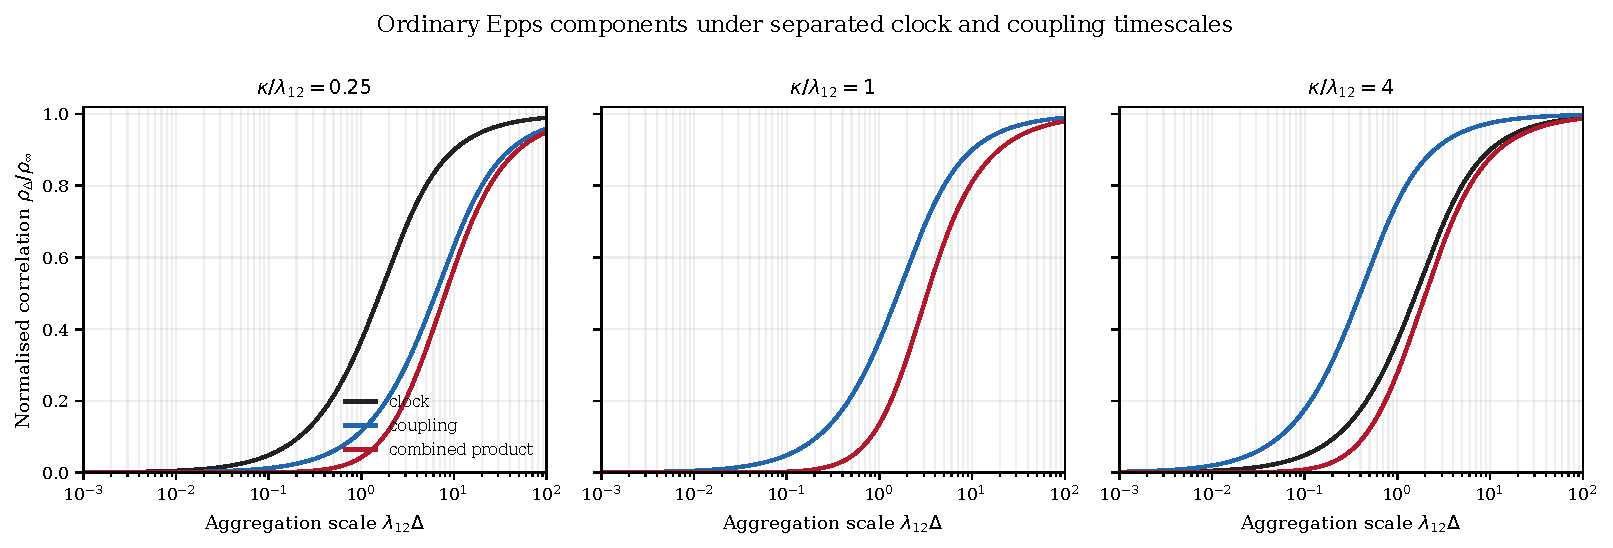
\includegraphics[width=\textwidth]{figures/figure-01-ordinary-epps-components-v1.pdf}
\caption{\textbf{Ordinary Epps components under separated clock and coupling timescales.} The clock curve is $F(\lambda_{12}\Delta)$, the coupling-response curve is $F(\kappa\Delta)$, and the combined curve is their separable product. The horizontal axis is aggregation scale in clock characteristic-time units and the vertical axis is $\rho_\Delta/\rho_\infty$. Panels use $\kappa/\lambda_{12}=0.25,1,4$, with $\lambda_{12}=1$ and $\rho_\infty=1$. The figure shows how the mechanisms contribute across separated and comparable timescales and supplies the analytic overlay baseline for v2.0.0. It supports the component decomposition under the paper's renewal-envelope and separability assumptions; it does not fit market data, simulate an order book, prove statistical independence, or establish the approximation outside those assumptions.}
\label{fig:ordinary-components}
\end{figure}

The short-scale limit of each component is linear in its dimensionless argument, so its rate elasticity approaches one. Once the component reaches its plateau, the elasticity approaches zero. For the product, the partial log-sensitivity to each rate is inherited from that component, while a common proportional perturbation of both rates has the sum of the two partial elasticities.

\begin{figure}[p]
\centering
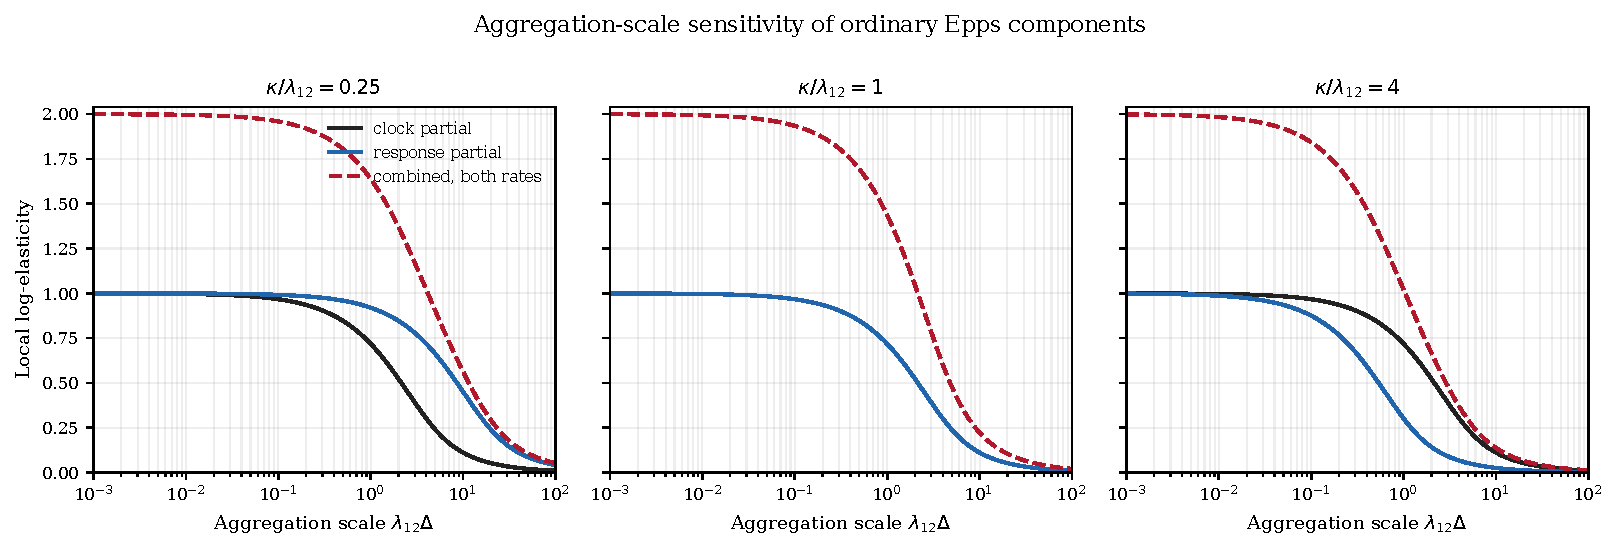
\includegraphics[width=\textwidth]{figures/figure-02-ordinary-epps-sensitivity-v1.pdf}
\caption{\textbf{Aggregation-scale sensitivity of ordinary Epps components.} Curves report $S_F(x)=xF'(x)/F(x)$ for clock refresh and coupling response. The dashed red curve is the log-sensitivity of the combined product when both rates receive the same proportional perturbation. Panels use the Figure~\ref{fig:ordinary-components} rate ratios. Sensitivity tends to one per component in the resolved short-scale limit and to zero on the long-scale plateau, locating the aggregation range that contains rate information. The figure supports local, model-conditional sensitivity statements; it is not a global-identifiability proof, an empirical uncertainty estimate, or evidence that either rate can be recovered without adequate short-scale observations.}
\label{fig:ordinary-sensitivity}
\end{figure}

The combined ordinary curve is invariant under exchange of the clock and response rates. Moreover,
\begin{equation}
C_{\mathrm{combined}}(\Delta)
=\frac{\lambda_{12}\kappa}{4}\Delta^2+O(\Delta^3)
\end{equation}
at short scale. Thus the leading combined curve alone reveals the rate product rather than assigning each timescale to its mechanism. The simulation results below therefore retain independently declared refresh and response rates.

\section{Fractional order sensitivity}

From Eq.~\eqref{eq:fractional},
\begin{equation}
F_\alpha(\Delta;\tau)
=\frac{(\Delta/\tau)^\alpha}{\Gamma(\alpha+2)}
+O(\Delta^{2\alpha}).
\end{equation}
A combined fractional curve therefore has leading power \(\Delta^{\alpha_c+\alpha_r}\). Equal-sum order pairs are deliberately included in Figure~\ref{fig:fractional} to show the resulting local confounding.

\begin{figure}[p]
\centering
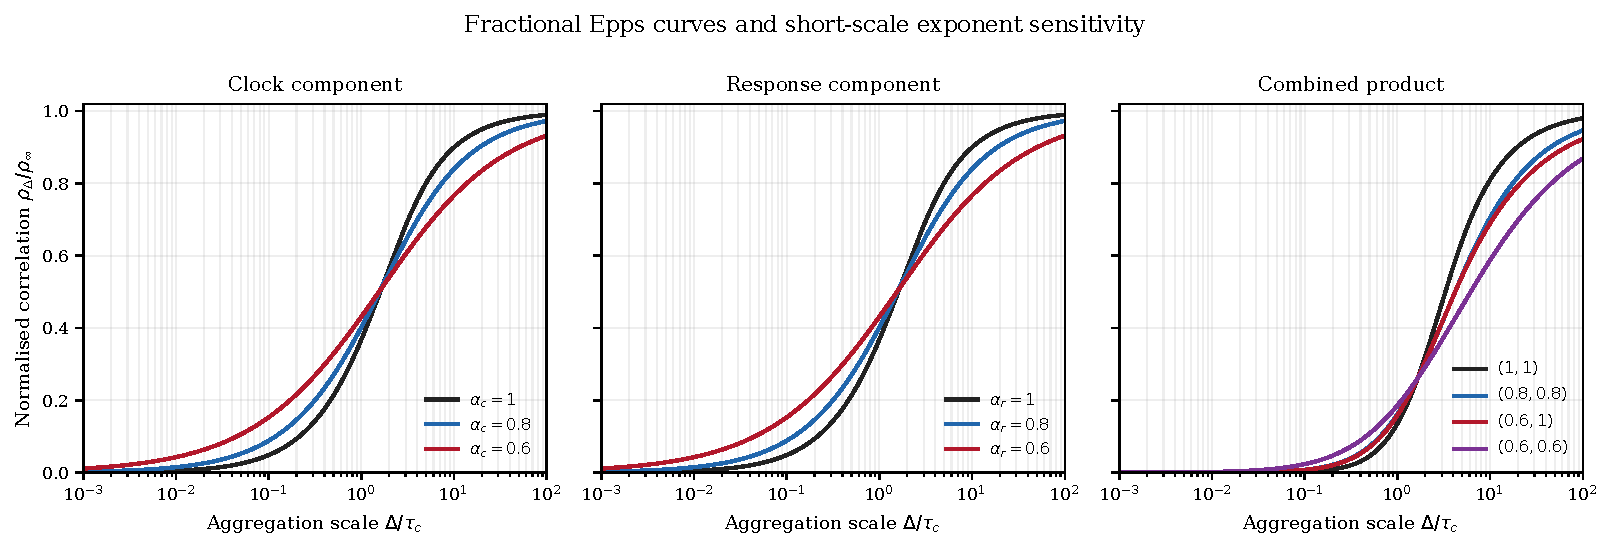
\includegraphics[width=\textwidth]{figures/figure-03-fractional-epps-sensitivity-v1.pdf}
\caption{\textbf{Fractional Epps curves and short-scale exponent sensitivity.} Clock and response components use Eq.~\eqref{eq:fractional}, with unit characteristic times and the diagnosed evaluator recorded in the numerical-design note; \(\alpha=1\) recovers the ordinary kernel. Combined curves use order pairs \((1,1),(0.8,0.8),(0.6,1),(0.6,0.6)\). The equal-sum cases \((0.8,0.8)\) and \((0.6,1)\) share leading short-scale power \(\Delta^{1.6}\), exposing local confounding even when later-scale curvature differs. The figure shows formula sensitivity to fractional order and the ordinary limit. It does not identify both orders from a combined curve alone, attach an unconditional ``slower'' interpretation across dimensional conventions, or validate a fractional market-clock mechanism empirically.}
\label{fig:fractional}
\end{figure}

\section{Conditional reaction-boundary propagation}

Equation~\eqref{eq:response} yields conditional log-elasticities $+1,+1,-1/2,-1$ with respect to coupling strength, source amplitude, source width, and front-slope magnitude. Figure~\ref{fig:boundary} changes one quantity at a time. This is a propagation experiment: multiple structural parameter combinations generate the same effective response rate and hence the same analytic Epps curve.

\begin{figure}[p]
\centering
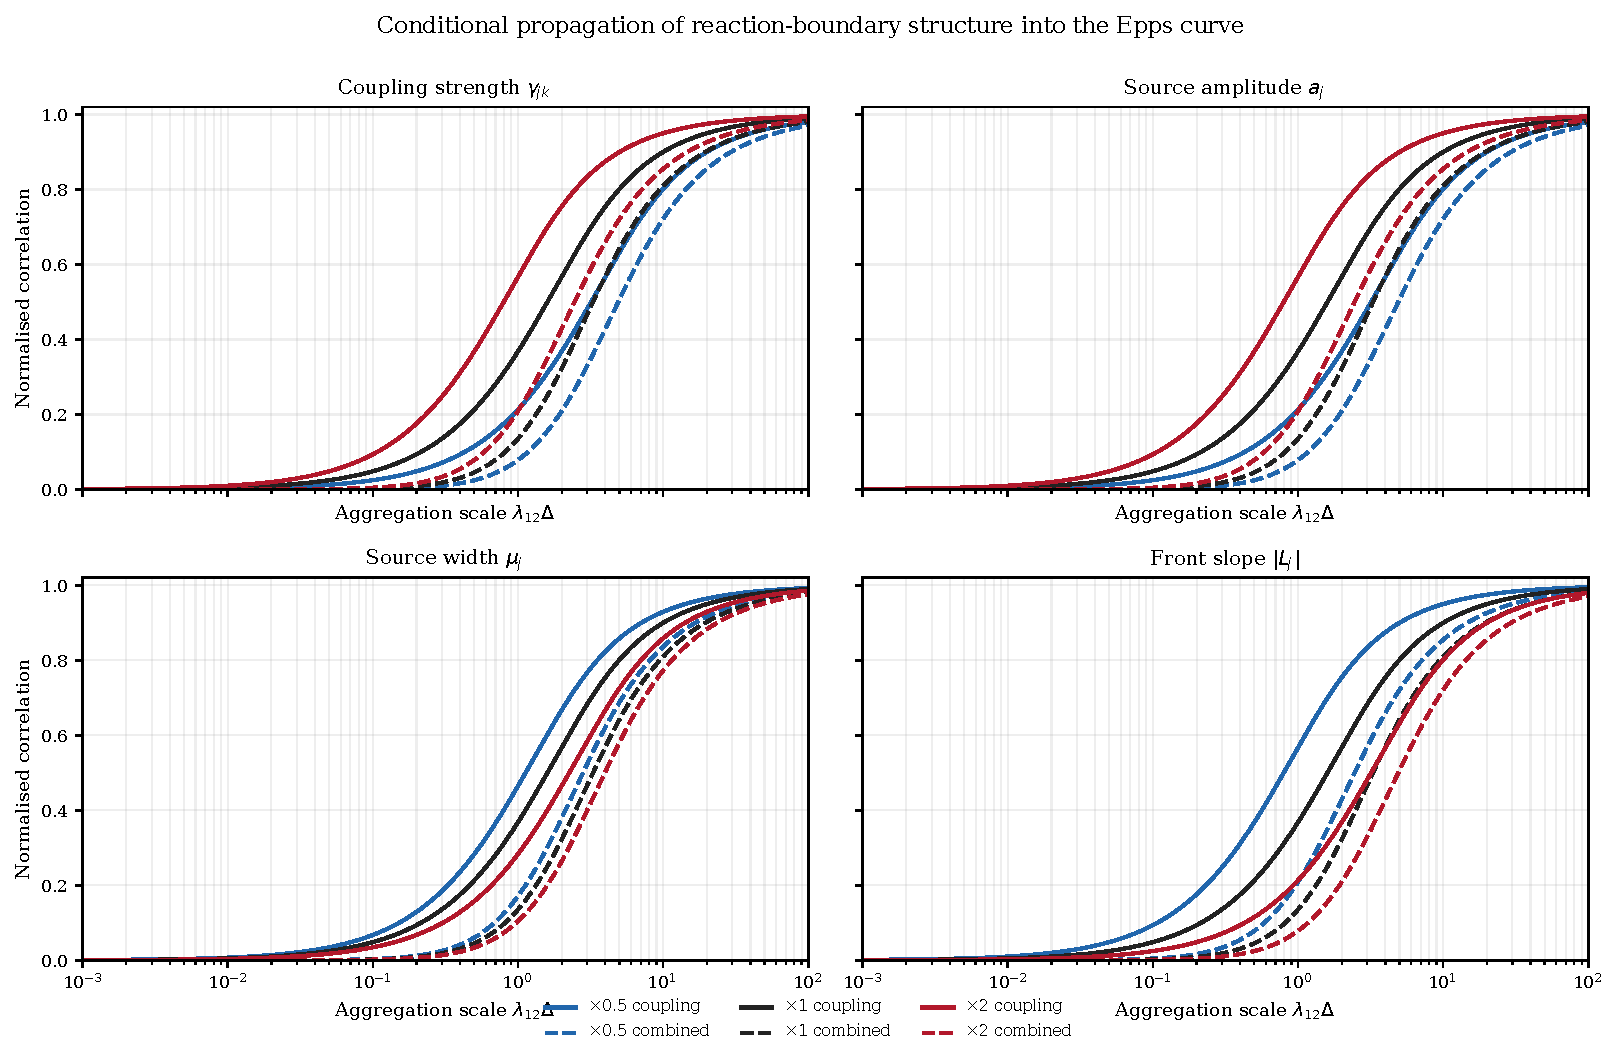
\includegraphics[width=\textwidth,height=0.72\textheight,keepaspectratio]{figures/figure-04-boundary-to-epps-propagation-v1.pdf}
\caption{\textbf{Conditional propagation of reaction-boundary structure into the Epps curve.} The response rate is varied through Eqs.~\eqref{eq:moment}--\eqref{eq:response}. Two symmetric books, unit source amplitude, width and front-slope magnitude, and $\gamma_{jk}=2/\sqrt\pi$ give baseline total response rate $\kappa=1$. Each panel changes one input by factors $0.5,1,2$, holding the others and the unit clock rate fixed; solid curves are coupling factors and dashed curves their combined products with the clock factor. This supports conditional propagation through the analytic response mapping. It does not uniquely infer reaction-front thickness, source width, or coupling strength from an Epps curve and does not claim pointwise equivalence to the legacy lattice coupling.}
\label{fig:boundary}
\end{figure}

Three distinct notions must not be collapsed into a single ``boundary thickness'': the local reaction-front slope \(|\mathcal L_j|\), the continuum selector regularisation \(\varepsilon\), and the lattice spacing \(\Delta x\). The first enters the structural response mapping. The second regularises side selection. The third is a numerical resolution parameter.

\section{Continuum selector and finite-grid representation}

The paper's smooth selector is
\begin{equation}
W(y,z;\varepsilon)=\frac12\left[1+\tanh\left(\frac{yz}{\varepsilon}\right)\right].
\end{equation}
For a centred symmetric full domain, \(yq_j(y)\) is even and the hyperbolic-tangent contribution is odd. Consequently the selected first moment is independent of \(\varepsilon\) in the continuum calculation. Finite domains, misaligned numerical selectors, and coarse grids can break this cancellation. Figure~\ref{fig:grid} diagnoses those representation effects and propagates them through an effective response rate.

\begin{figure}[p]
\centering
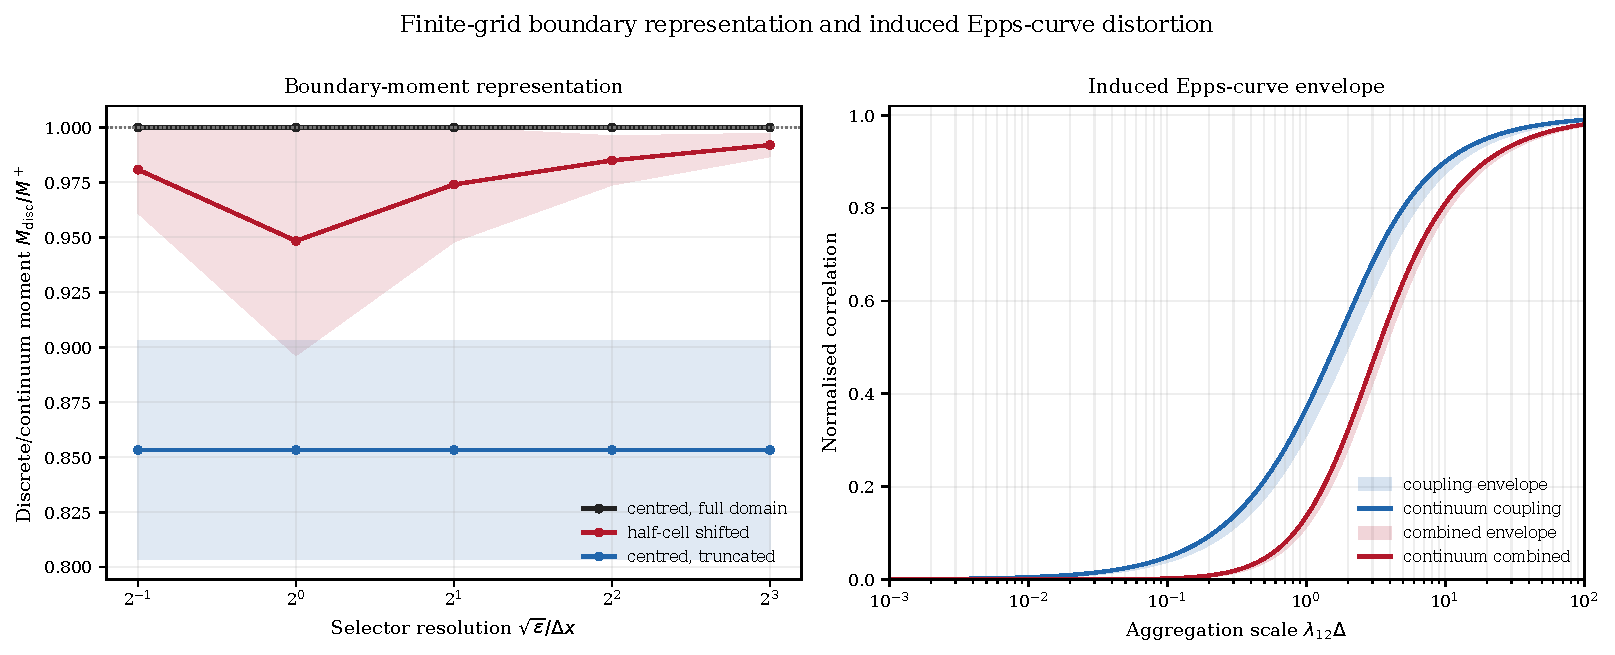
\includegraphics[width=\textwidth]{figures/figure-05-finite-grid-epps-distortion-v1.pdf}
\caption{\textbf{Finite-grid boundary representation and induced Epps-curve distortion.} The left panel reports discrete-to-continuum first-moment ratios as selector resolution \(\sqrt\varepsilon/\Delta x\), lattice spacing, selector alignment, and domain margin vary. Lines give the midpoint and bands the range over four lattice spacings. The centred full-domain case is the parity control; half-cell selector displacement and truncation measure numerical representation errors. The right panel propagates all diagnosed effective-rate ratios through the coupling and combined Epps formulas; lines are continuum baselines and bands are discrete-representation envelopes. Structural parameters are fixed. The figure supports convergence and numerical-sensitivity statements and defines resolution metadata required for v2 overlays. It does not introduce a new continuum Epps mechanism or treat selector width, lattice spacing, and reaction-front thickness as interchangeable.}
\label{fig:grid}
\end{figure}

\clearpage
\section{Calendar-time representation and memory diagnostic}

The aggregation variable in Figures~\ref{fig:ordinary-components}--\ref{fig:grid} remains the observation-window lag, but is reported relative to the clock characteristic time. Writing
\begin{equation}
x=\lambda_{12}\Delta t=\frac{\Delta t}{\tau_c},
\qquad \tau_c=\lambda_{12}^{-1},
\end{equation}
shows that a calendar-time presentation requires only a declared time convention. For an ordinary exponential memory with rate \(r\),
\begin{equation}
h_r(u)=e^{-ru},
\qquad
F(r\Delta t)=1-\frac{1}{\Delta t}\int_0^{\Delta t}h_r(u)\,du.
\label{eq:memory-average}
\end{equation}
For the clock mechanism, \(h_{\lambda_{12}}\) is the no-refresh survival. For the coupling mechanism, \(h_\kappa\) is the relaxation survival and equals the normalised positive-lag exponential covariance kernel used in the paper. Figure~\ref{fig:calendar-bridge} therefore presents the same analytical factors as Figure~\ref{fig:ordinary-components}, not a new Epps mechanism.

\begin{figure}[p]
\centering
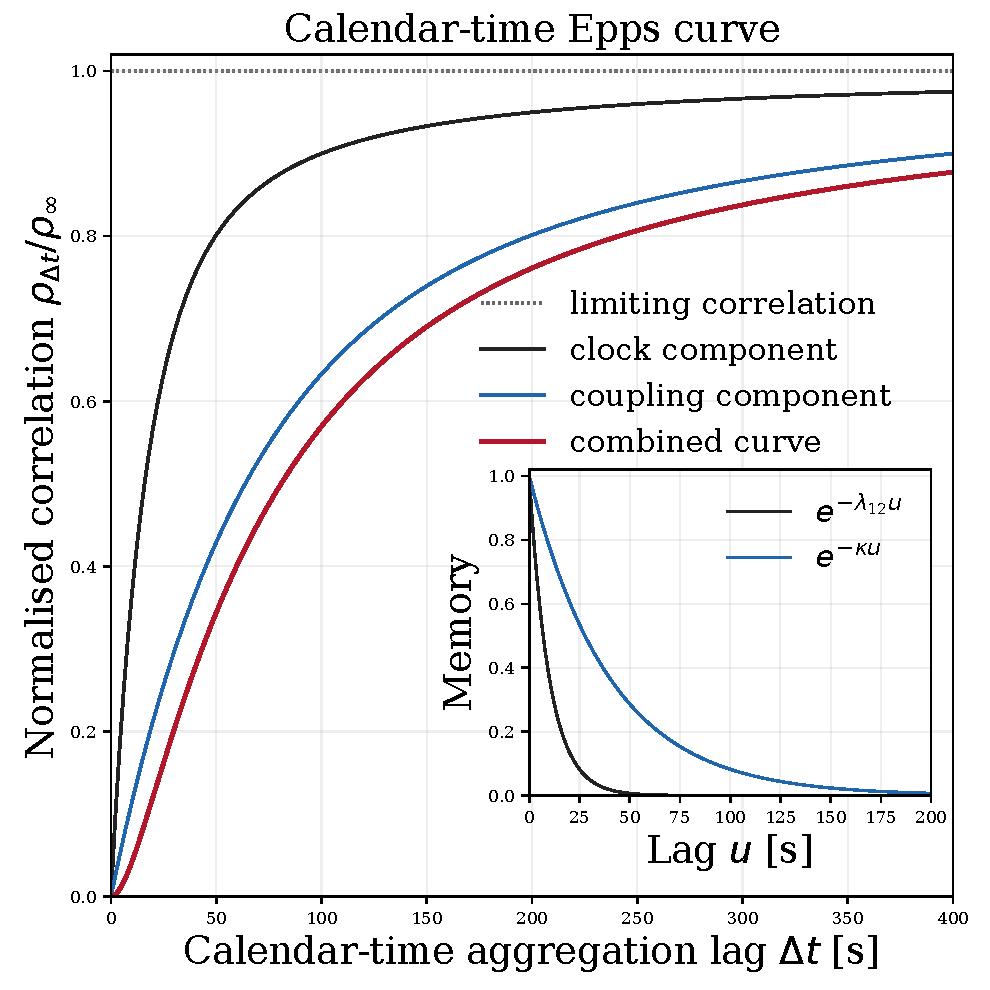
\includegraphics[width=0.91\textwidth]{figures/figure-06-calendar-time-epps-memory-v1.pdf}
\caption{\textbf{Calendar-time Epps curve.} The square main panel rewrites the Figure~\ref{fig:ordinary-components} slow-response profile on a linear calendar-time axis using the explicitly illustrative convention $\lambda_{12}=0.1\,\mathrm{s}^{-1}$, $\kappa=0.025\,\mathrm{s}^{-1}$, and $\rho_\infty=1$, corresponding to $\tau_c=10$ s and $\tau_r=40$ s. Black, blue and red curves are the clock factor, coupling factor and their leading-order separable product; the grey dotted line marks the normalised limiting correlation $\rho_{\Delta t}/\rho_\infty=1$. The enlarged inset reports $h_c(u)=e^{-\lambda_{12}u}$ and $h_r(u)=e^{-\kappa u}$: respectively the no-refresh survival and coupling-relaxation survival, with the latter also equal to the normalised positive-lag exponential covariance kernel. The seconds scale is not fitted to data, and the inset is neither a path autocorrelation nor a power-spectrum estimate. Path-derived autocorrelations are reported separately in Figure~\ref{fig:dependence}.}
\label{fig:calendar-bridge}
\end{figure}

The distinction from the simulation output is substantive. A sample autocorrelation requires a generated path, a declared estimator and finite-sample uncertainty. The deterministic inset exposes only the memory functions that enter Eq.~\eqref{eq:memory-average}. Figure~\ref{fig:dependence} reports the separate path-derived log-mid increment and trade-sign autocorrelations without retrospectively relabelling this analytical diagnostic.

\clearpage
\section{Uniform-operational simulation}

Let \(u_n=n\Delta u\) be the common operational grid. Both density fields are
advanced on this grid before any calendar observation is constructed. External
innovations are book-specific, the translation-mode coupling uses
Eq.~\eqref{eq:translation-mode}, and labelled order events modify the density
state at declared operational steps. The boundary price is the accepted unique
interior zero crossing of the signed density field.

For book \(j\), let \(\tau_{j,m}\) be its completed calendar refresh events.
The software first selects the latest event at or before \(t\), then the latest
uniform operational node at or before that event:
\begin{equation}
m_j(t)=\max\{m:\tau_{j,m}\leq t\},
\qquad
n_j(t)=\max\{n:u_n\leq\tau_{j,m_j(t)}\},
\qquad
P_j^{\rm cal}(t)=P_j^{\rm op}(u_{n_j(t)}).
\label{eq:subordination}
\end{equation}
Equation~\eqref{eq:subordination} is previous-refresh subordination. It selects
an already completed state and never changes an operational update interval.

% Audited algorithmicx presentation for the v2.1.0 computational supplement.

\subsection{Executable numerical algorithms}
\label{app:numerical-algorithms}

Algorithms~\ref{alg:operational-translation-simulation}--
\ref{alg:paired-clock-impact} make the software's two time layers explicit.
Operational evolution uses one frozen pre-step state; renewal generation and
calendar observation act only on completed paths.  Every coupled update reads
the same frozen histories, and every shocked/control comparison uses the same
realised clock.

\begin{algorithm}[H]
\caption{Coupled operational-time reaction-boundary evolution}
\label{alg:operational-translation-simulation}
\begin{algorithmic}[1]
\Require Uniform grid $x_i$, step $\Delta u$, histories
$\{\varphi_m^{i(j)}\}_{m\leq n}$, and boundaries $p_n^{(j)}$
\Require Sources $s_n^{i(j)}$, event fields $\delta_n^{i(j)}$, and directed
rates $\kappa_{jk}\geq0$
\Ensure Next densities and boundaries, coupling/source fields, and diagnostics
\State Freeze $\varphi_{n,\mathrm{pre}}^{i(j)}\gets\varphi_n^{i(j)}$ and
$p_{n,\mathrm{pre}}^{(j)}\gets p_n^{(j)}$ for every book
\ForAll{ordered pairs $j\leftarrow k$}
  \State $z_{jk,n}\gets p_{n,\mathrm{pre}}^{(j)}-p_{n,\mathrm{pre}}^{(k)}$
  \State $v_{j,n}^{\Delta x}\gets-\partial_x^{\Delta x}
  \varphi_{n,\mathrm{pre}}^{(j)}$; set its outer values to zero
  \State $\ell_{T,n}^{i(j,k)}\gets-\kappa_{jk}z_{jk,n}
  v_{j,n}^{\Delta x}(x_i)$
\EndFor
\ForAll{books $j$}
  \State $\ell_{T,n}^{i(j)}\gets\sum_{k\ne j}\ell_{T,n}^{i(j,k)}$
  \State $c_n^{i(j)}\gets s_n^{i(j)}+\delta_n^{i(j)}+
  \ell_{T,n}^{i(j)}$
  \State $\varphi_{n+1,\mathrm{raw}}^{(j)}\gets
  \mathcal U_{\Delta u}^{(j)}[\{\varphi_m^{(j)}\}_{m\leq n},c_n^{(j)}]$
  \State Impose $\varphi_{n+1}^{0(j)}=\varphi_{n+1}^{I(j)}=0$
  \State Form the admissible exact-zero and strict-crossing set
  $\mathcal Z_{n+1}^{(j)}$ defined below
  \State Require $\mathcal Z_{n+1}^{(j)}\ne\varnothing$ and set
  $p_{n+1}^{(j)}\gets\mathcal B_j[\mathcal Z_{n+1}^{(j)};p_n^{(j)}]$
\EndFor
\State \textbf{return} states, boundaries, candidate data, fields, sources,
and recurrence contributions
\end{algorithmic}
\end{algorithm}

Here $\mathcal U_{\Delta u}^{(j)}$ is the fixed-step DTRW recurrence; the
additive field $c_n^{(j)}$ enters its source channel rather than forming a
separate update.  The boundary candidates used in the algorithm are
\begin{align}
\mathcal Z_{n+1,\mathrm{exact}}^{(j)}
&=\left\{x_i:1\leq i\leq I-1,\ \varphi_{n+1}^{i(j)}=0,\
\varphi_{n+1}^{i-1(j)}\varphi_{n+1}^{i+1(j)}<0,\
|L_i^{(j)}|\geq L_{\min}\right\},\\
\mathcal Z_{n+1,\mathrm{cross}}^{(j)}
&=\left\{x_i-\frac{\varphi_{n+1}^{i(j)}}{L_{i+1/2}^{(j)}}:\
\varphi_{n+1}^{i(j)}\varphi_{n+1}^{i+1(j)}<0,\
|L_{i+1/2}^{(j)}|\geq L_{\min}\right\},
\end{align}
with
\begin{equation}
L_i^{(j)}=\frac{\varphi_{n+1}^{i+1(j)}-\varphi_{n+1}^{i-1(j)}}{2\Delta x},
\qquad
L_{i+1/2}^{(j)}=\frac{\varphi_{n+1}^{i+1(j)}-\varphi_{n+1}^{i(j)}}{\Delta x}.
\end{equation}
The full set is their union.  Unique selection requires one candidate;
nearest-previous selection requires a unique minimum distance from $p_n^{(j)}$
and rejects distance ties.  Either $\kappa_{jk}=0$ or $z_{jk,n}=0$ makes the
corresponding directed field exactly zero.

\begin{algorithm}[H]
\caption{Book-specific previous-refresh calendar observation}
\label{alg:previous-refresh-observation}
\begin{algorithmic}[1]
\Require Completed prices $p^{(j)}(u_n)$ on a uniform operational grid
\Require Strict refresh paths $0=\tau_{j,0}<\cdots<\tau_{j,M_j}$,
nondecreasing queries $t_r$, and integer lags $h_q$
\Ensure Calendar prices, index/support records, pooled components, and
optional conditional moments
\State Require $0\leq t_0\leq\cdots\leq t_R\leq
\min\{u_N,\tau_{1,M_1},\tau_{2,M_2}\}$
\ForAll{books $j$ and queries $t_r$}
  \State $m_j(t_r)\gets\max\{m:\tau_{j,m}\leq t_r\}$
  \State $n_j(t_r)\gets\max\{n:u_n\leq\tau_{j,m_j(t_r)}\}$
  \State $P_\Delta^{(j)}(t_r)\gets p^{(j)}(u_{n_j(t_r)})$
\EndFor
\ForAll{lags $h_q$ and admissible origins $t_r$}
  \State Form $R_{q,r}^{(j)}\gets
  P_\Delta^{(j)}(t_{r+h_q})-P_\Delta^{(j)}(t_r)$
  \State Accumulate $R_{q,r}^{(1)}R_{q,r}^{(2)}$ and
  $(R_{q,r}^{(j)})^2$ into $S_q^{12}$ and $S_q^{jj}$
  \State Record $J_{j,q,r}=(a_j,b_j]$ and overlap $\Theta_{q,r}$
  \If{the symmetric reduced conditional reference is requested}
    \State Evaluate $K_{q,r}$, $C_{q,r}^{12}$, and $V_{q,r}^{(j)}$ below
  \EndIf
\EndFor
\State Pool component sums across path groups, then compute
$\widehat\rho_q=S_q^{12}/\sqrt{S_q^{11}S_q^{22}}$
\State Form delete-one-group ratios and the path-group jackknife error
\State \textbf{return} observations, indices, support, components, ratios,
and uncertainty
\end{algorithmic}
\end{algorithm}

The nested map in lines 2--4 is the exact previous-completed-state inverse: it
first selects a refresh event and then an operational node, without
interpolation, extrapolation, or terminal-state clamping.  For each return,
\begin{equation}
(a_1,b_1,a_2,b_2)=\Delta u\,
\bigl(n_1(t_r),n_1(t_{r+h_q}),n_2(t_r),n_2(t_{r+h_q})\bigr),
\qquad
\Theta_{q,r}=\max\{0,\min(b_1,b_2)-\max(a_1,a_2)\}.
\end{equation}
When requested, the symmetric conditional reference uses
$\kappa=\kappa_{12}+\kappa_{21}>0$ and
\begin{align}
K_{q,r}&=e^{-\kappa|b_1-b_2|}-e^{-\kappa|b_1-a_2|}
-e^{-\kappa|a_1-b_2|}+e^{-\kappa|a_1-a_2|},\\
C_{q,r}^{12}&=\Theta_{q,r}-\frac{K_{q,r}}{2\kappa},
\label{eq:algorithm-conditional-cross}\\
V_{q,r}^{(j)}&=(b_j-a_j)
-\frac{e^{-\kappa(b_j-a_j)}-1}{\kappa}.
\label{eq:algorithm-conditional-variance}
\end{align}
The final minus sign is intentional: $e^{-\kappa d}-1\leq0$, so the
Ornstein--Uhlenbeck spread contribution adds to marginal variance and subtracts
from cross-covariance.  Identity clocks recover the implemented coupling-only
moments to the registered tolerance.

For $G$ independent path groups, uncertainty uses
\begin{equation}
\widehat\rho_q^{(-g)}=
\frac{S_q^{12}-S_{gq}^{12}}
{\sqrt{(S_q^{11}-S_{gq}^{11})(S_q^{22}-S_{gq}^{22})}},
\qquad
\operatorname{se}_{\mathrm{JK}}(\widehat\rho_q)=
\left[\frac{G-1}{G}\sum_{g=1}^{G}
\left(\widehat\rho_q^{(-g)}-\overline\rho_q^{(-)}\right)^2\right]^{1/2}.
\end{equation}

\begin{algorithm}[H]
\caption{Mittag--Leffler and exponentially tempered renewal paths}
\label{alg:renewal-clock-construction}
\begin{algorithmic}[1]
\Require Order $0<\beta\leq1$, scale $\tau>0$, horizon $T>0$, and independent
open uniforms $(U_r,V_r,E_r,A_r)$ supplied by the caller
\Require Optional tempering rate $\lambda_T>0$
\Ensure Strict renewal events $0=\tau_0<\cdots<\tau_M$ with $\tau_M\geq T$
\For{$r=1,2,\ldots$ until the retained cumulative wait reaches $T$}
  \If{$\beta=1$}
    \State $S_r\gets1$
  \Else
    \State $\theta_r\gets\pi U_r$ and $Z_r\gets-\log V_r$
    \State $S_r\gets
    \dfrac{\sin(\beta\theta_r)}{\sin(\theta_r)^{1/\beta}}
    \left[\dfrac{\sin((1-\beta)\theta_r)}{Z_r}\right]^{(1-\beta)/\beta}$
  \EndIf
  \State $W_r\gets\tau(-\log E_r)^{1/\beta}S_r$
  \If{untempered or $A_r\leq e^{-\lambda_TW_r}$}
    \State Append $W_r$ and its cumulative sum to the renewal path
  \EndIf
\EndFor
\State \textbf{return} event times, retained waits, law parameters, stream id,
and supported horizon
\end{algorithmic}
\end{algorithm}

Algorithm~\ref{alg:renewal-clock-construction} is exact for the declared
Laplace transforms in Eqs.~\eqref{eq:ml-wait-laplace} and
\eqref{eq:tempered-ml-laplace}.  It neither clips heavy waits nor rescales the
accepted sample to a target mean.  At $\beta=1$ the untempered construction
reduces to exponential waiting intervals with mean $\tau$.

\begin{algorithm}[H]
\caption{Common-input paired impact under an observation clock}
\label{alg:paired-clock-impact}
\begin{algorithmic}[1]
\Require Completed control paths $P_{p,j}^{0}(u_n)$ and signed-event shocked
paths $P_{p,b,s,j}^{1}(u_n)$ generated from identical initial states and inputs
\Require One book-specific renewal pair per path, event step $n_e$, and lags
$\ell_q$ on the query grid
\Ensure Own/cross impact means, path standard errors, and active fractions
\ForAll{paths $p$}
  \State Apply Algorithm~\ref{alg:previous-refresh-observation} to the control
  path and retain its selected indices $n_{p,j}(t)$
  \ForAll{event books $b$ and signs $s\in\{-1,+1\}$}
    \State Apply the \emph{same} realised clock pair to the shocked path
    \ForAll{response books $j$ and lags $\ell_q$}
      \State $I_{p,b,s,j}(\ell_q)\gets s[P_{p,b,s,j}^{1,c}(t_e+\ell_q)
      -P_{p,j}^{0,c}(t_e+\ell_q)]$
      \State $A_{p,j}(\ell_q)\gets
      \mathbf 1\{n_{p,j}(t_e+\ell_q)\geq n_e\}$
    \EndFor
  \EndFor
\EndFor
\State Average signs within path, then paths and exchange-symmetric own/cross
book pairs; compute standard errors across paths
\State \textbf{return} impact curves and active-observation fractions
\end{algorithmic}
\end{algorithm}

For a meta-order, line 7 is evaluated at each child step and at declared lags
after the final child; activity at relaxation lag is measured relative to the
final child.  An inactive observation contributes its actual paired value,
normally zero before the event is observed, rather than being removed by
conditioning.

Algorithm~\ref{alg:operational-translation-simulation} owns dynamics and
boundary extraction.  Algorithms~\ref{alg:previous-refresh-observation} and
\ref{alg:renewal-clock-construction} own observation only, while
Algorithm~\ref{alg:paired-clock-impact} owns the estimand.  This separation is
the principal control for the Poisson, Mittag--Leffler and tempered
observation-clock comparisons.


\subsection{Final theory-to-simulation Epps comparison}

Figure~\ref{fig:final-epps} is the primary release result. The component inputs,
clock paths, holdout structure and parameter values were fixed before the
combined comparison. The leading-order product remains the analytical paper
envelope. The same-clock conditional reference is the exact finite-step
conditional moment evaluated at the operational indices selected by the same
realised clocks as the simulation; it is not a fitted replacement.

\begin{figure}[p]
\centering
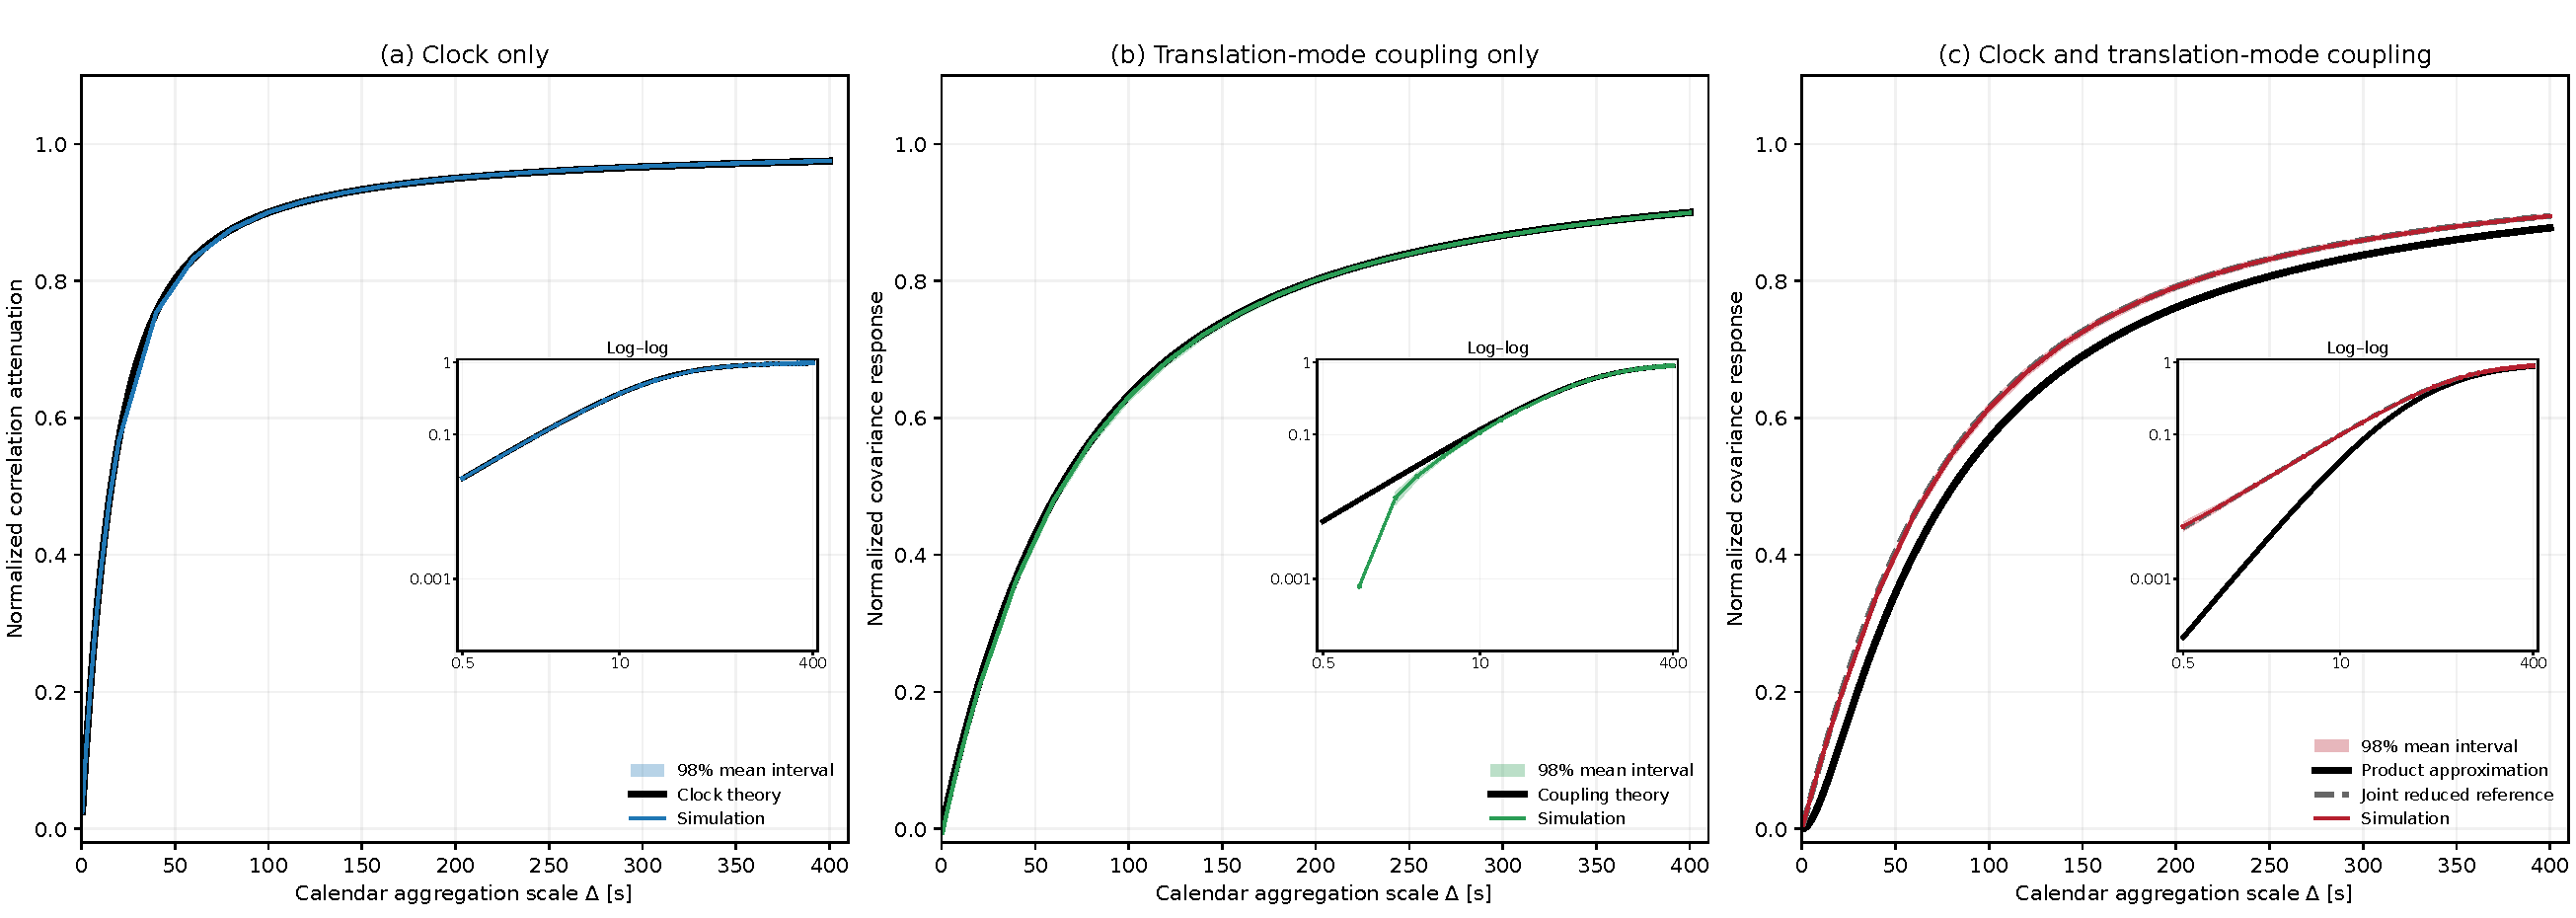
\includegraphics[width=\textwidth]{figures/figure-07-final-estimator-aware-epps-v2.pdf}
\caption{\textbf{Clock, coupling and combined Epps curves: theory and simulation.} The three square panels share one linear 0--400 second and 0--1.1 normalized-covariance scale. Panel (a) compares the clock-only simulation with the exact equal-rate previous-refresh factor $F(\lambda^{\rm clk}\Delta)$, where each book has $\lambda^{\rm clk}=0.1\,\mathrm{s}^{-1}$ rather than the $0.2\,\mathrm{s}^{-1}$ pooled minimum-wait rate. Panel (b) compares the translation-mode coupling simulation with $F(\kappa\Delta)$, using $\kappa=0.025\,\mathrm{s}^{-1}$. Panel (c) compares the combined no-refit holdout with the paper's leading-order separable product $F(\lambda^{\rm clk}\Delta)F(\kappa\Delta)$ and the same-clock conditional reference. The latter evaluates the reduced finite-step conditional moment at the same realised previous-refresh indices as the simulation; it is not a fitted curve. Its combined RMSE is 0.039719, standardized RMSE is 0.455132, and pointwise normal-band coverage is complete. No parameter, normalization or time map is refitted.}
\label{fig:final-epps}
\end{figure}

\subsection{Translation-mode component}

The translation-mode coupling is tested separately under identity clocks before it is
used in the combined route. Deterministic signed-front relaxations diagnose the
registered response rate; stochastic holdout paths test normalized covariance
and the distinct finite-scale return correlation. The covariance scale is
frozen from a disjoint calibration ensemble.

\begin{figure}[p]
\centering
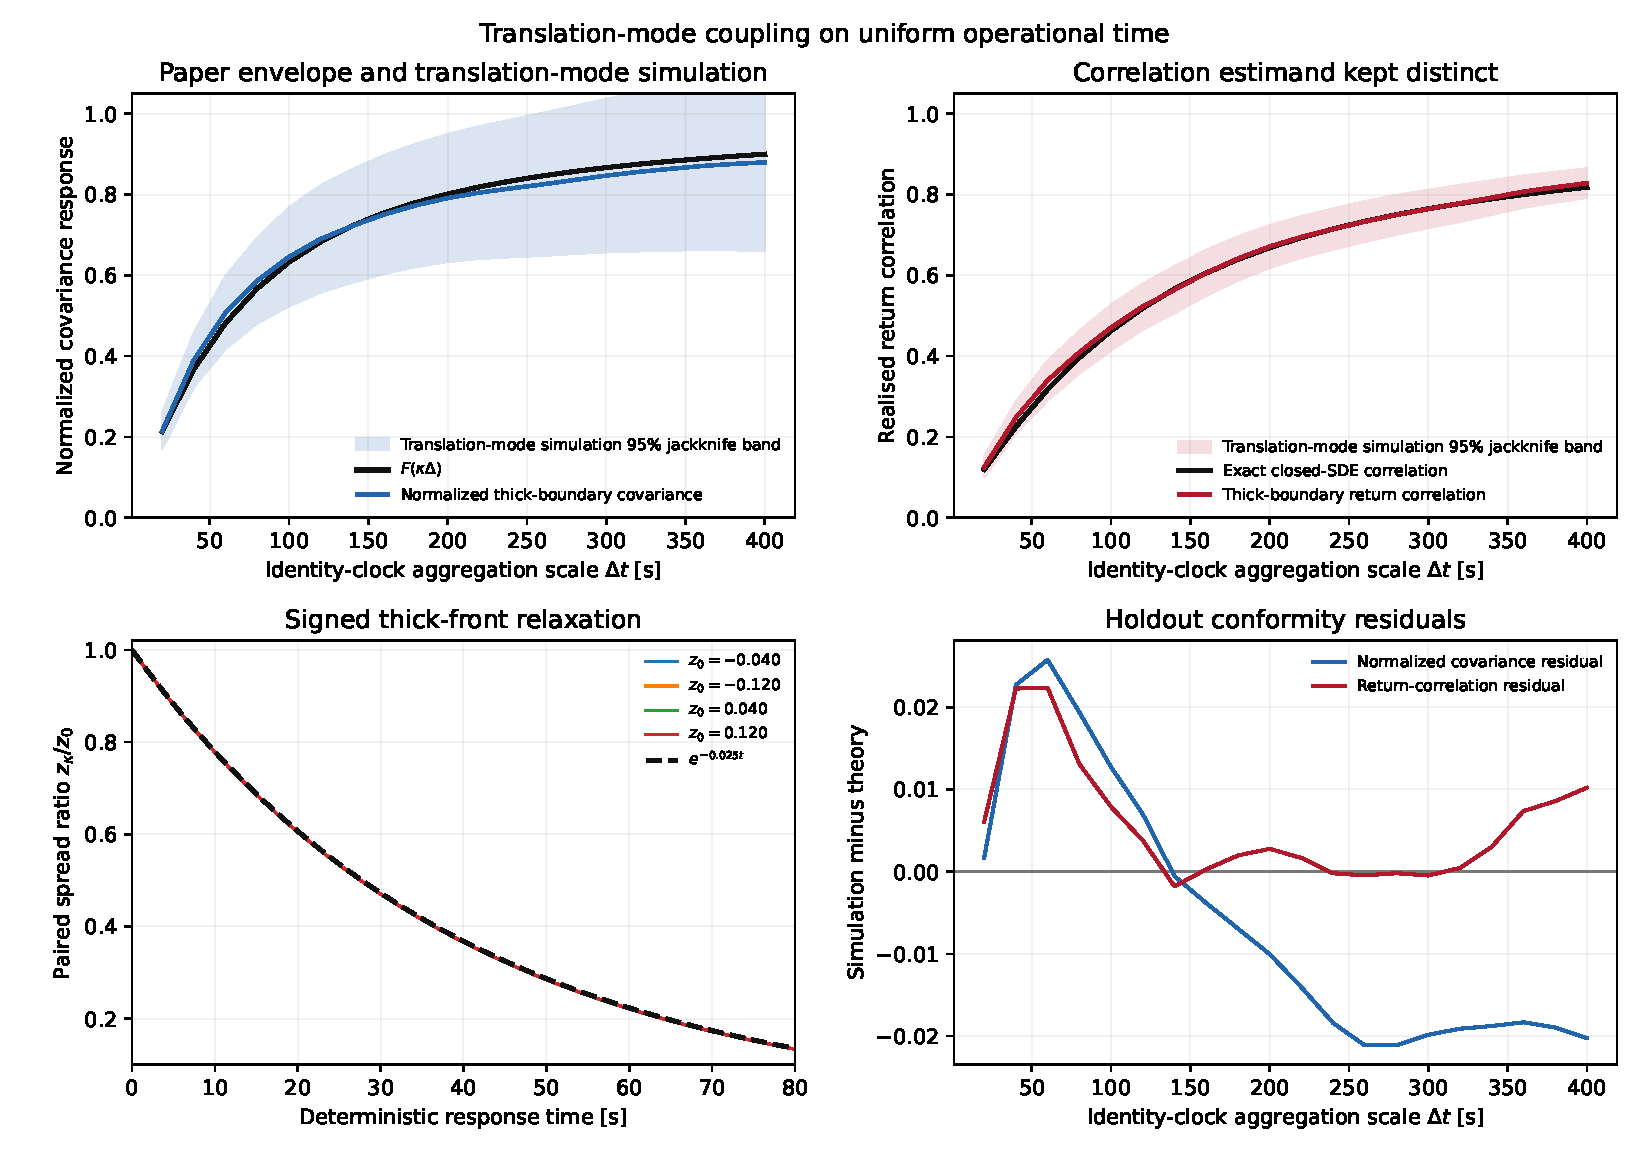
\includegraphics[width=\textwidth]{figures/figure-08-corrected-translation-mode-coupling-v2.pdf}
\caption{\textbf{Translation-mode coupling on uniform operational time.} Holdout thick-boundary paths are compared with the analytical normalized covariance response and the distinct finite-scale return correlation. Lower panels verify signed deterministic front relaxation and residuals at the frozen response rate. No clock, interpolation or parameter fit enters this component gate.}
\label{fig:translation-mode-coupling}
\end{figure}

\section{Event impact and dependence diagnostics}

Market-order events consume opposing density at the active boundary and are
recorded on an immutable event tape. Impact is measured by pairing each event
path with an otherwise identical zero-input control. Responses are
aggressor-signed log-boundary differences, so own and cross effects use one
common linear scale. Calendar versions are obtained only after the operational
paths are complete, using Eq.~\eqref{eq:subordination}.

\begin{figure}[p]
\centering
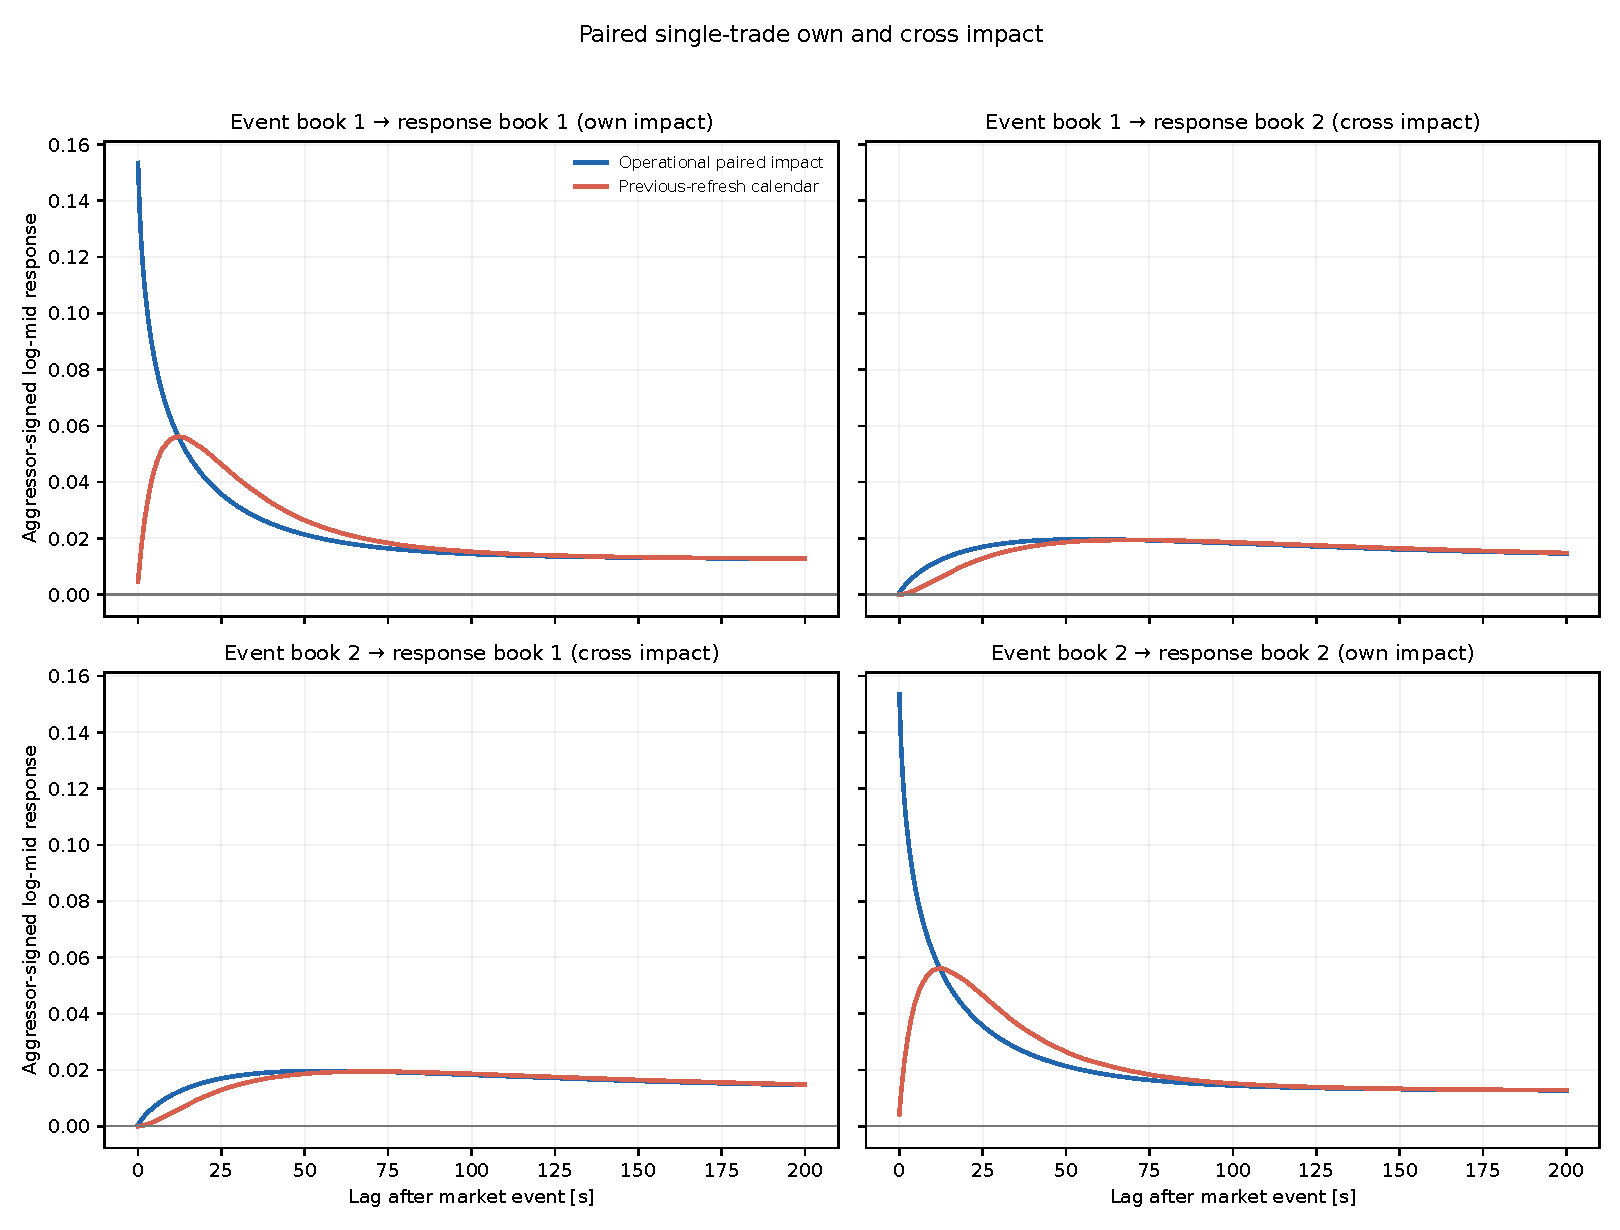
\includegraphics[width=\textwidth]{figures/figure-09-single-trade-impact-v2.pdf}
\caption{\textbf{Paired single-trade own and cross impact.} One labelled market order is compared with a matched control in operational and previous-refresh calendar views. The figure reports own and cross boundary responses on a common linear scale. It is a declared model experiment, not an empirical trade calibration.}
\label{fig:single-trade}
\end{figure}

A meta-order is a declared schedule of child market orders with fixed total
quantity and book. Equal-volume horizon comparisons distinguish schedule timing
from a true participation rate, which would require background market-order
volume not present in this model.

\begin{figure}[p]
\centering
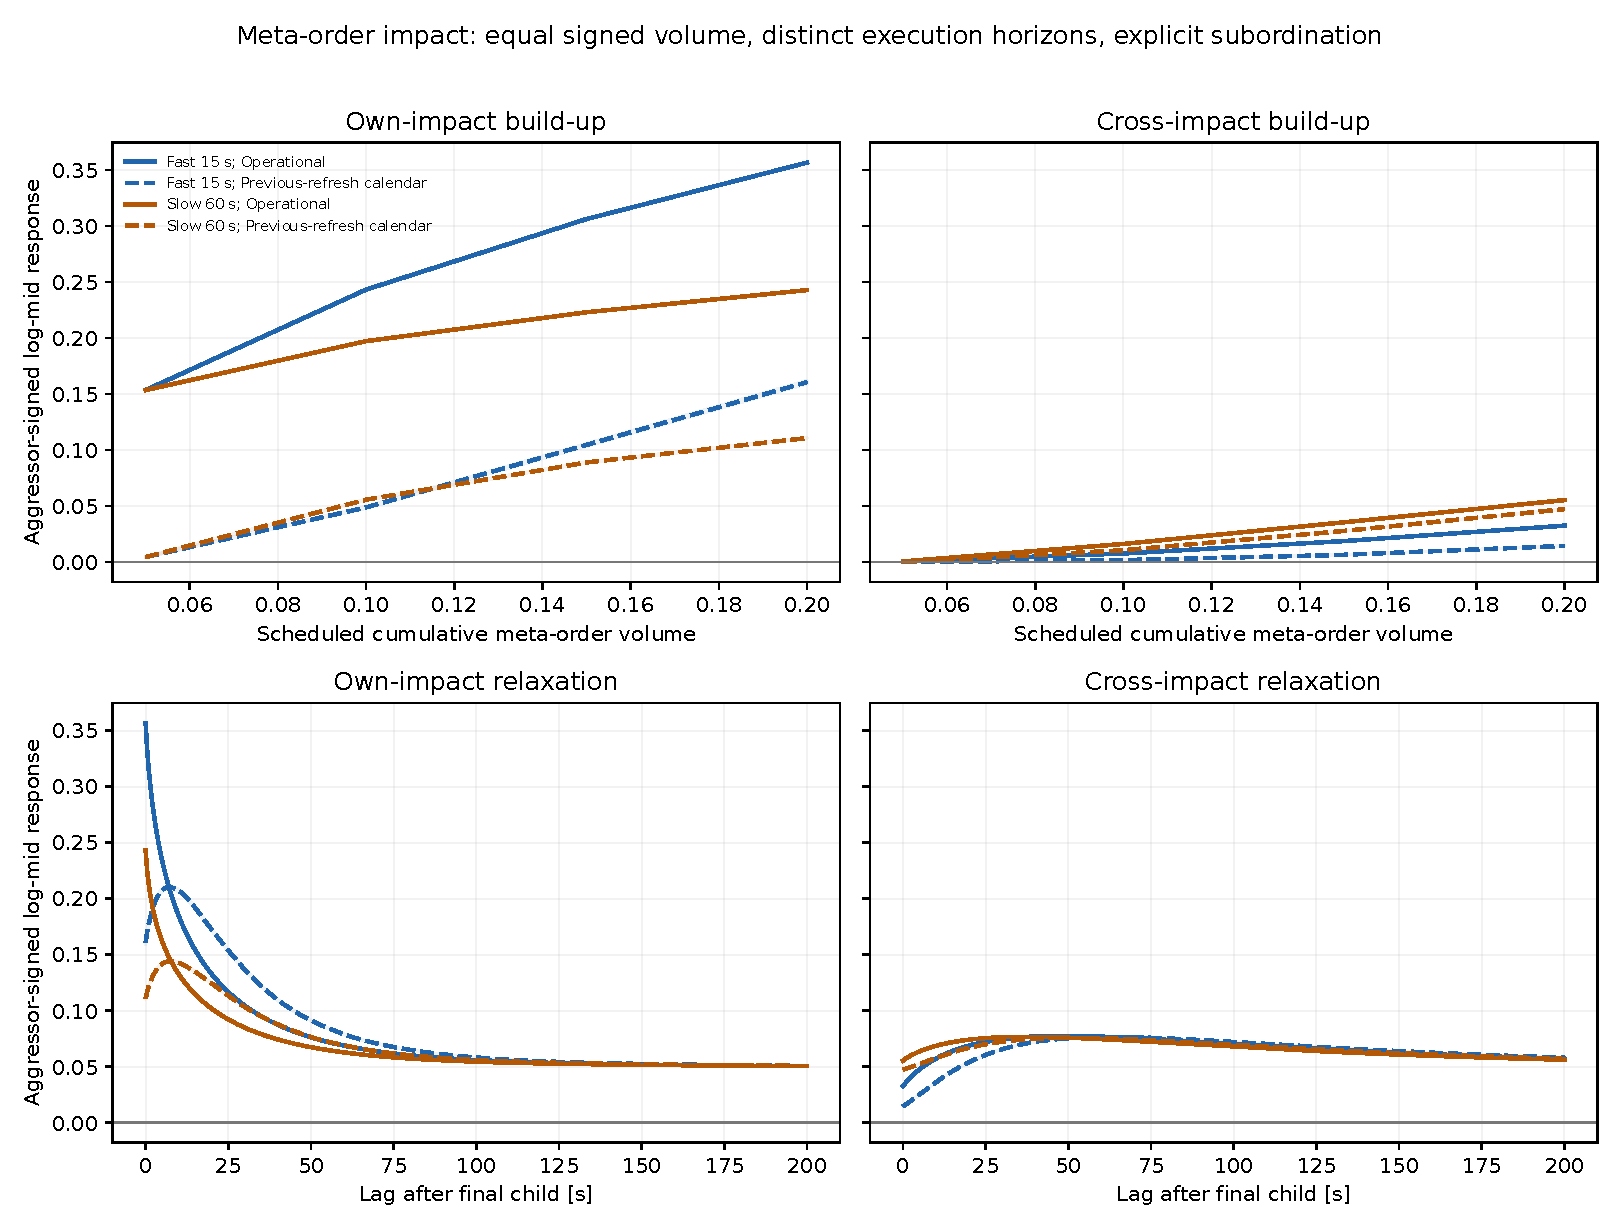
\includegraphics[width=\textwidth]{figures/figure-10-meta-order-impact-v2.pdf}
\caption{\textbf{Scheduled meta-order own and cross impact.} Matched schedules report trajectory, peak, relaxation and equal-volume horizon comparisons under operational and explicitly subordinated calendar observations. Schedule timing, cross-impact catch-up and long-lag convergence are kept as distinct observables.}
\label{fig:meta-order}
\end{figure}

For a sequence \(X_n\), let \(\bar X_{L,k}\) and \(\bar X_{R,k}\) denote the
separate sample means of \(\{X_n\}_{n=1}^{N-k}\) and
\(\{X_{n+k}\}_{n=1}^{N-k}\).  The registered positive-lag statistic is the
Pearson correlation of those two overlapping slices,
\begin{equation}
\widehat\rho_X(k)=
\frac{\sum_{n=1}^{N-k}\bigl(X_n-\bar X_{L,k}\bigr)
\bigl(X_{n+k}-\bar X_{R,k}\bigr)}
{\sqrt{\left[\sum_{n=1}^{N-k}\bigl(X_n-\bar X_{L,k}\bigr)^2\right]
\left[\sum_{n=1}^{N-k}\bigl(X_{n+k}-\bar X_{R,k}\bigr)^2\right]}},
\qquad \widehat\rho_X(0)=1.
\label{eq:pearson-slice-acf}
\end{equation}
The price statistic is applied to log-mid increments, never to price levels.
Trade-sign diagnostics distinguish ground-truth aggressor signs, a
quote/midpoint rule and the historically inherited tick rule. Event-time signs
and calendar-binned signed flow are separate estimands.

\begin{figure}[p]
\centering
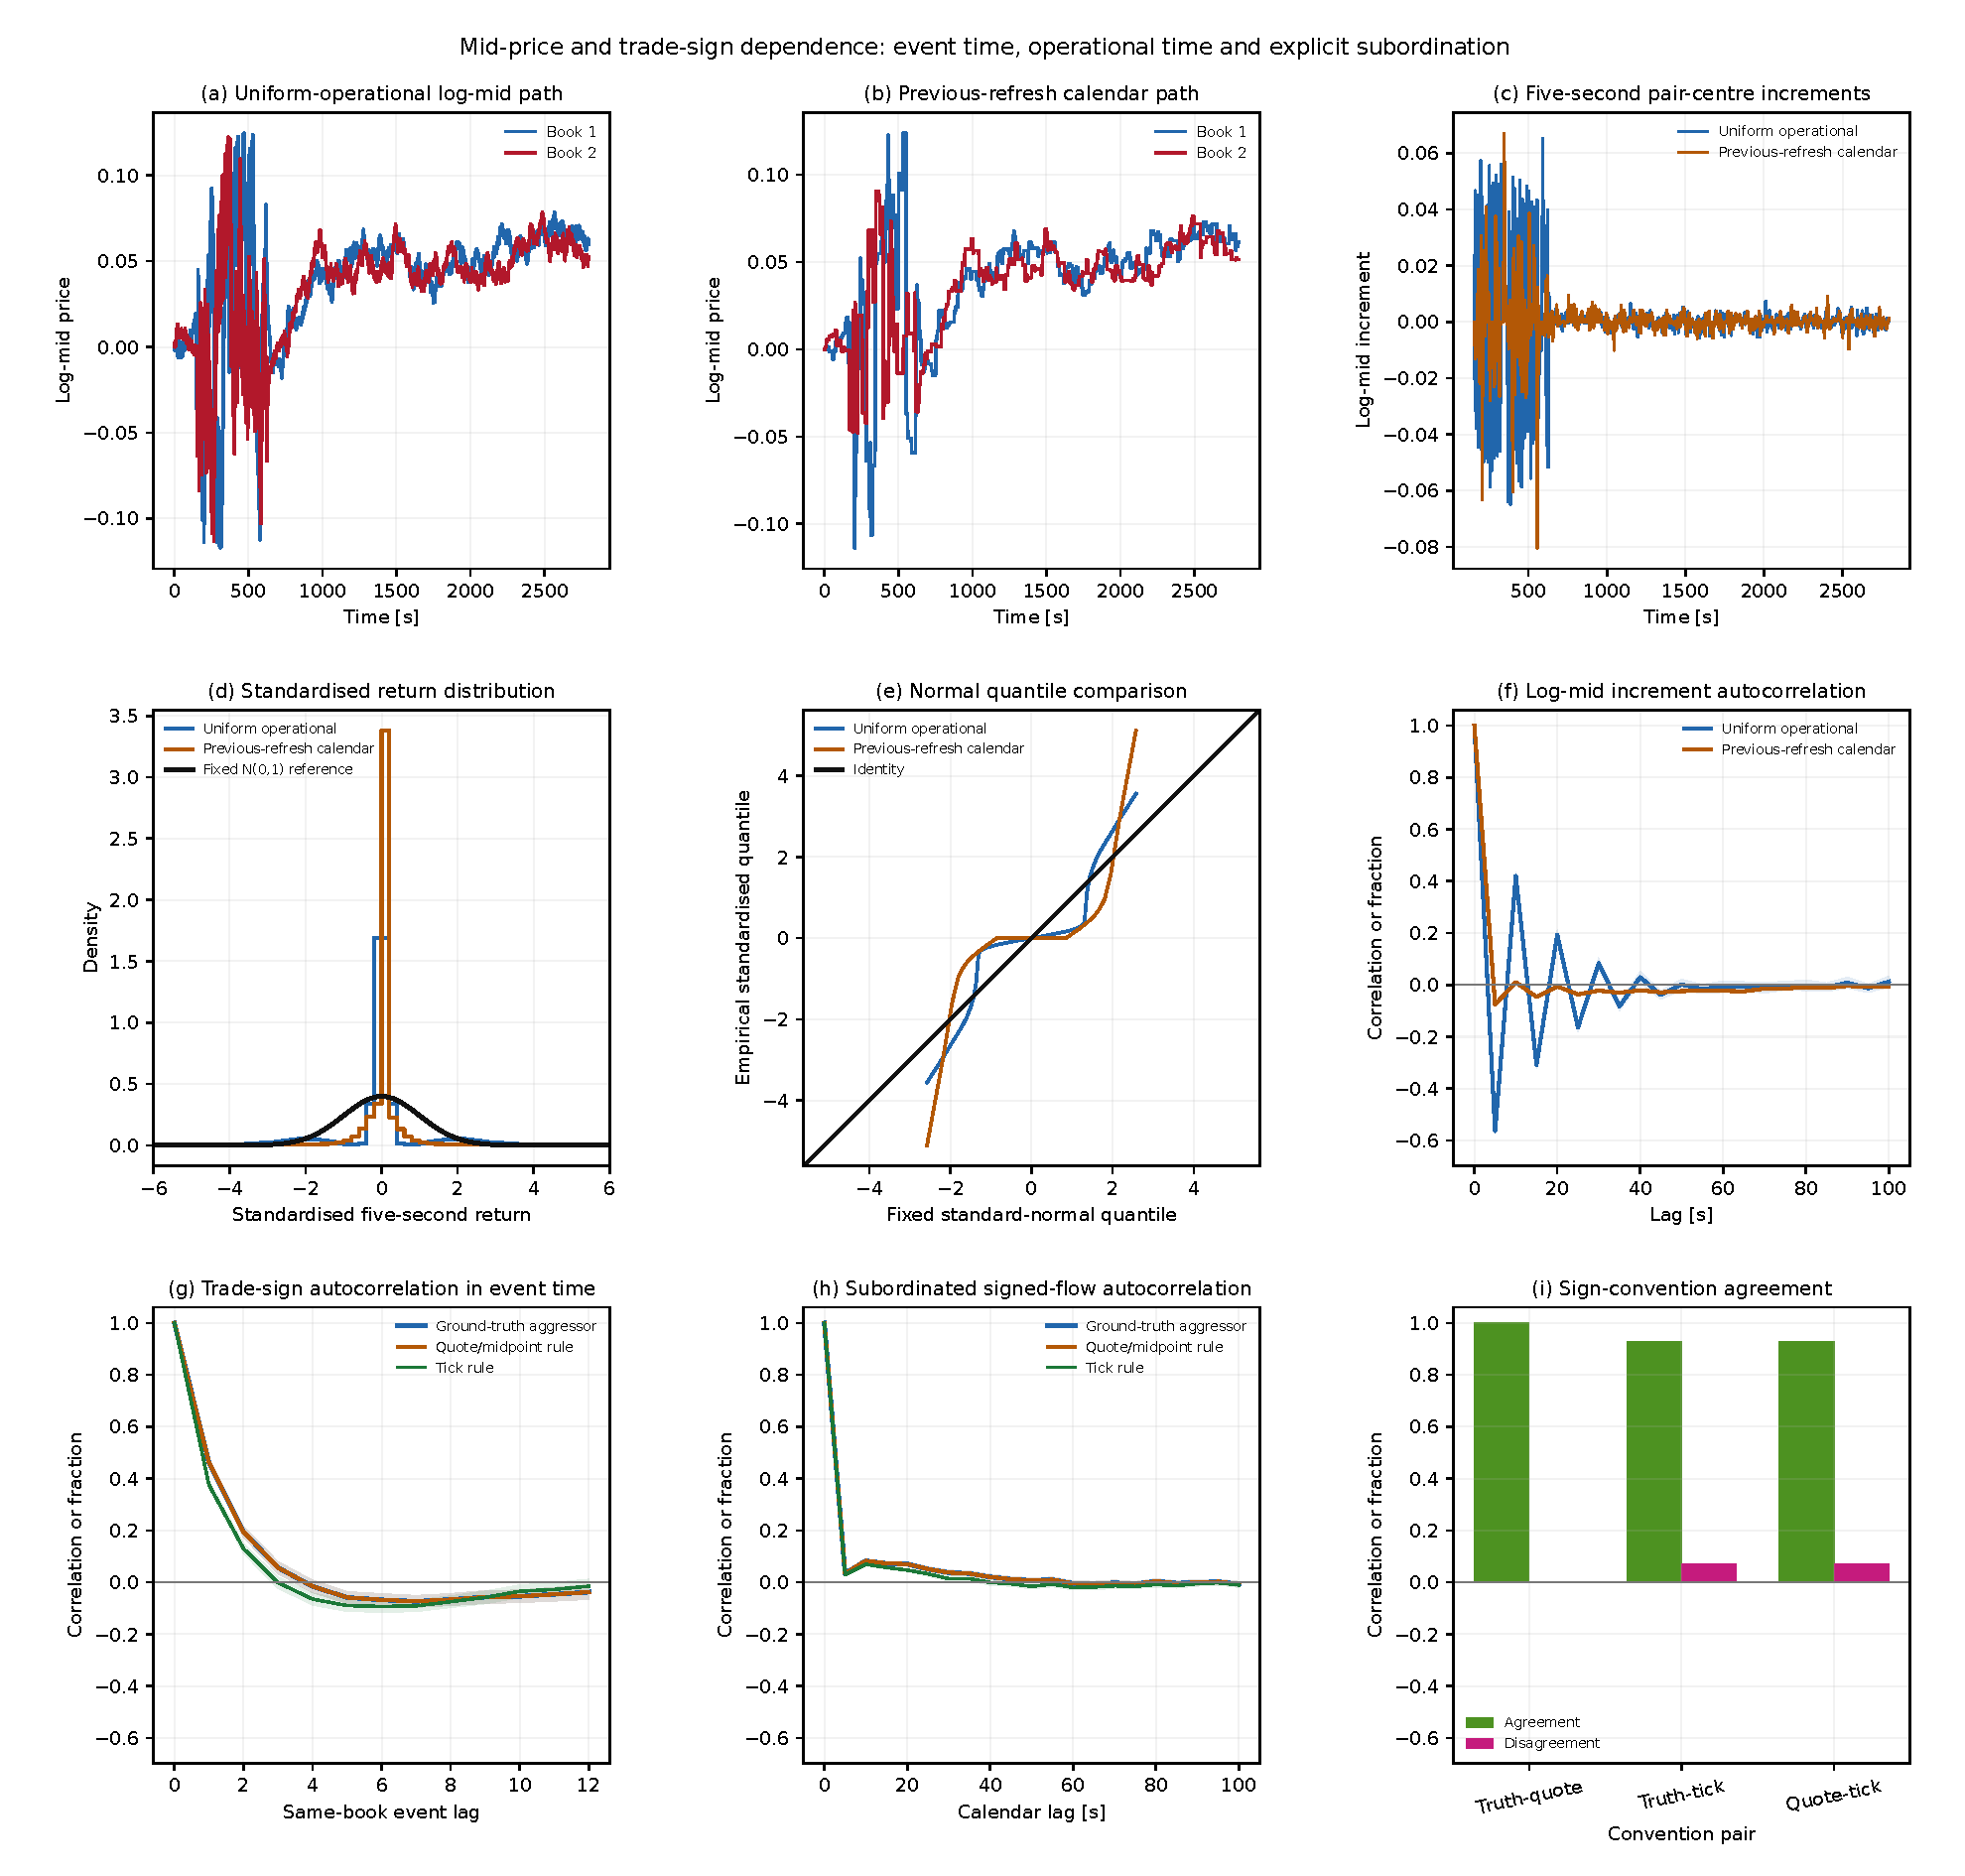
\includegraphics[width=\textwidth]{figures/figure-11-mid-price-trade-sign-autocorrelations-v2.pdf}
\caption{\textbf{Mid-price and trade-sign autocorrelations.} Panels report log-mid increment autocorrelation for uniform operational and previous-refresh calendar observations, same-book event-time trade-sign autocorrelation for three sign conventions, subordinated signed-flow autocorrelation, and sign-convention agreement. Price-level autocorrelation is excluded. The finite Markov persistence is an estimator fixture, not empirical calibration or an endogenous long-memory claim. The operational five-second ACF is a registered finite periodic-schedule diagnostic, and its detailed curve is phase-sensitive to that schedule.}
\label{fig:dependence}
\end{figure}

% Figure 12 supplementary-material insert for the v2.1.0 development gate.
% The published v2.0.0 supplement and accepted source-v1 paper remain frozen.

\subsection{Fixed-time order-book shock recovery}
\label{app:fixed-time-shock-recovery}

Figure~\ref{fig:fixed-time-shock-recovery} follows one buy market order in
book 1 through the current fixed-grid operational dynamics.  Immediately
before the declared operational step, the order consumes opposing density
from the reaction boundary outwards.  If $M_{1,n_*}$ denotes the resulting
density increment, then
\begin{equation}
  \varphi^+_{1,n_*}=\varphi^-_{1,n_*}+M_{1,n_*},
  \qquad
  \Delta x\sum_i |M_{1,n_*,i}|=Q.
\end{equation}
The event is applied once and only to book 1.  The second book remains active
through the receiving-front translation-mode coupling, although its density
and the coupling contribution are not separately drawn.

For a completed operational step the stored density satisfies
\begin{equation}
  \varphi_{j,n+1}
  =H_{j,n}+\varphi^+_{j,n}+C_{j,n}+A_{j,n}+L_{j,n}+B_{j,n},
\end{equation}
where $H$ is the transport or memory contribution,
\begin{equation}
  A_{j,n}=\Delta u\,q_j,
  \qquad
  C_{j,n}=\left(e^{-\nu_j\Delta u}-1\right)\varphi^+_{j,n},
  \qquad
  L_{j,n}=\Delta u\,\ell_{j\leftarrow k},
\end{equation}
and $B$ is the imposed outer-boundary correction.  The plotted arrivals,
removals and market-order impulse are density contributions rather than rates.
All are drawn on the same density scale.  In particular, the green curve is
$A_{j,n}=\Delta u\,q_j$ and is small relative to $\varphi_j$ because
$\Delta u=0.005$; it is not independently rescaled.  The unplotted terms are
retained in the machine-readable ledger.

Two differences from Bauer et al. Figure 2 follow from the present model.  The
accepted configuration has $\nu_1=\nu_2=0$, so $C_{j,n}=0$ and the gold
removal curve is identically zero.  It is retained to preserve the plotted
object map; no positive cancellation rate is introduced for visual agreement.
Second, boundary-outward consumption produces a short zero-density interval in
the intermediate $0^+$ state.  That state has no unique simple zero crossing.
The marker in panel (b) is therefore the last registered boundary $p_1^-$;
the first completed fixed-grid step restores a unique registered reaction
boundary.  Later markers are independently recovered from the corresponding
density states.

The first completed step gives an own-boundary displacement of $0.0997$ in
log-price units.  The displacement reaches $0.111$ at $2$ seconds and then
decreases to $0.0160$ at $80$ seconds.  Thus the computed late state is
substantially relaxed but remains displaced from the matched control over the
displayed horizon.

The calculation uses fixed $\Delta x=0.1$ and $\Delta u=0.005$ model-time
units, with $100$ seconds per model-time unit.  Innovations are set to zero so
that the chronology isolates event consumption, diffusion, source renewal and
coupling.  A matched no-event control remains in the numerical checks but is
not added to the nine-panel figure.  The result recovers the structure and
scientific question of the earlier figure; it does not assert numerical
identity with its non-uniform-time trajectory or parameterisation.

\begin{figure}[p]
\centering
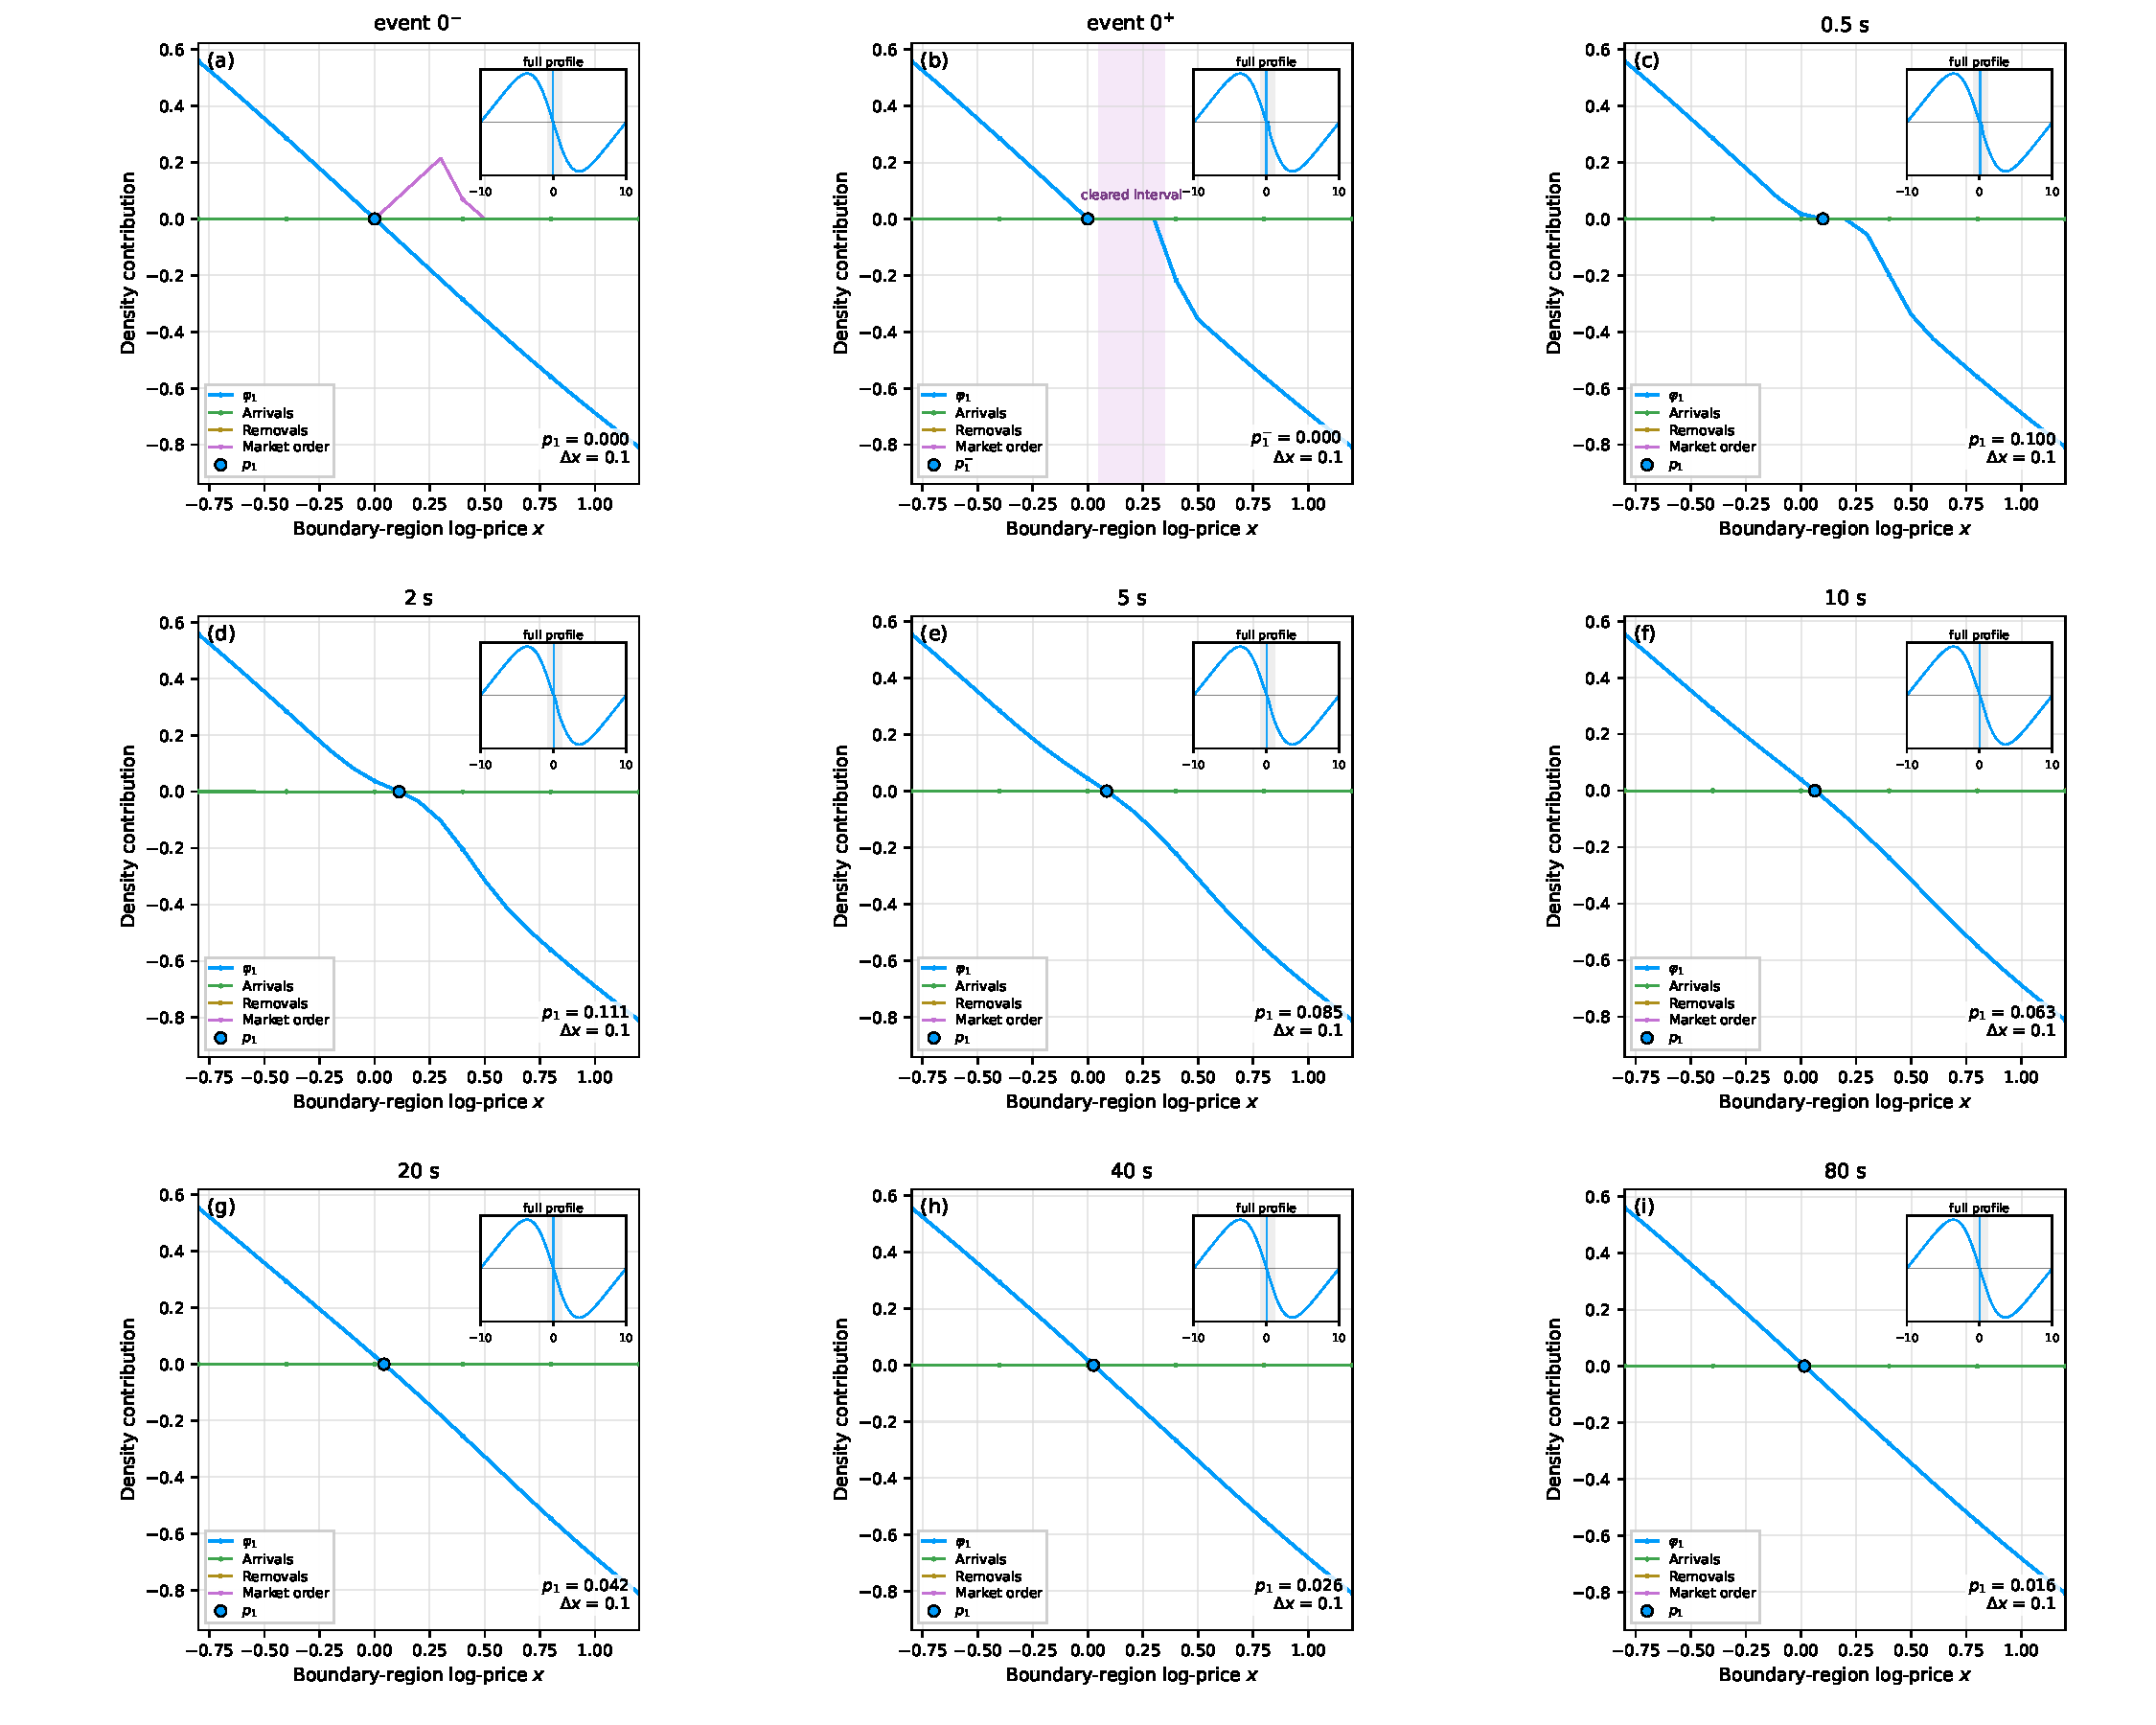
\includegraphics[width=\textwidth]{figures/figure-12-order-book-shock-recovery-v2.pdf}
\caption{\textbf{Fixed-time order-book shock recovery.} Nine snapshots follow
a buy market order in book 1 from the pre-event state $0^-$, through the
post-consumption state $0^+$, to $80$ seconds of fixed operational-time
evolution.  Blue is the signed density $\varphi_1$, green is the per-step
arrival contribution, gold is the per-step removal contribution, magenta is
the market-order density increment shown in panel (a), and the blue marker is the registered
reaction boundary.  The order consumes opposing liquidity from the boundary
outwards.  In panel (b) this creates a zero-density interval, so the marker is
the last registered boundary $p_1^-$; a unique simple zero is again registered
after the first completed step.  The accepted model has $\nu_1=\nu_2=0$, and
the gold curve is consequently zero in every panel.  Translation-mode coupling
to book 2 remains active and is retained in the numerical ledger but is not
drawn as an additional curve.  The registered boundary moves by $0.0997$ after
the first completed step, reaches $0.111$ at $2$ seconds and relaxes to a
residual displacement of $0.0160$ at $80$ seconds.  The price grid and
operational step are fixed.  All contribution curves use the same density
scale and are not independently rescaled.
The figure recovers the earlier panel structure without claiming a pointwise
replication of the Bauer et al. trajectory.}
\label{fig:fixed-time-shock-recovery}
\end{figure}


\clearpage
% Figure 13 supplementary-material insert for the v2.1.0 development gate.
% The published v2.0.0 supplement and accepted source-v1 paper remain frozen.

\subsection{Stylised facts under operational and calendar observation}
\label{app:stylised-facts-recovery}

Figure~\ref{fig:stylised-facts-recovery} retains the panel hierarchy of Bauer
et al. as a structural reference while changing the estimands to match the
current theory and available provenance.  The earlier figure compares
empirical data with a calibrated non-uniform-time legacy implementation.  The
present figure compares one current-model ensemble before and after a separate
previous-refresh observation map.  The operational model evolves on a fixed
grid; calendar non-uniformity enters only through subordination.  Log-mid
displacement is reported relative to the translation-invariant zero origin,
so its level cannot be compared with the arbitrary price levels in the legacy
figure.

The production event process uses irregular background market-order arrivals
at the declared mean rate.  Event quantity is fixed from the full-experiment
event/background displacement scale rather than from the earlier impact-test
quantity.  No smoothing, path selection or parameter refit is used.  The
accepted ensemble contains 16 paths and 5,600 operational steps per path; the
extension from 2,800 steps was required to obtain at least 25 operational
observations beyond $|z|>3$ under the registered tail gate.

The distinction between the two rows explains the principal morphological
difference.  The operational row has no zero-return atom and is close to
Gaussian for the registered baseline.  The calendar row holds the last
available value between refreshes, creating 60.49\% zero five-second
increments, a central density spike, an extended QQ plateau and larger
standardised tails.  These are observation-clock effects; they do not imply
that the underlying operational path has changed.

The baseline uses ordinary operational order $\alpha_u=1$, zero cancellation
and a Poisson refresh clock.  It therefore does not test fractional
operational memory or non-Markovian calendar waiting times.  Those mechanisms
remain distinct in the Angstmann--Gebbie formulation and require their own
registered numerical controls before use.  Signed-order-flow persistence is
imposed by the declared finite-persistence aggressor-sign input and is not an
endogenous model result.

\begin{figure}[p]
\centering
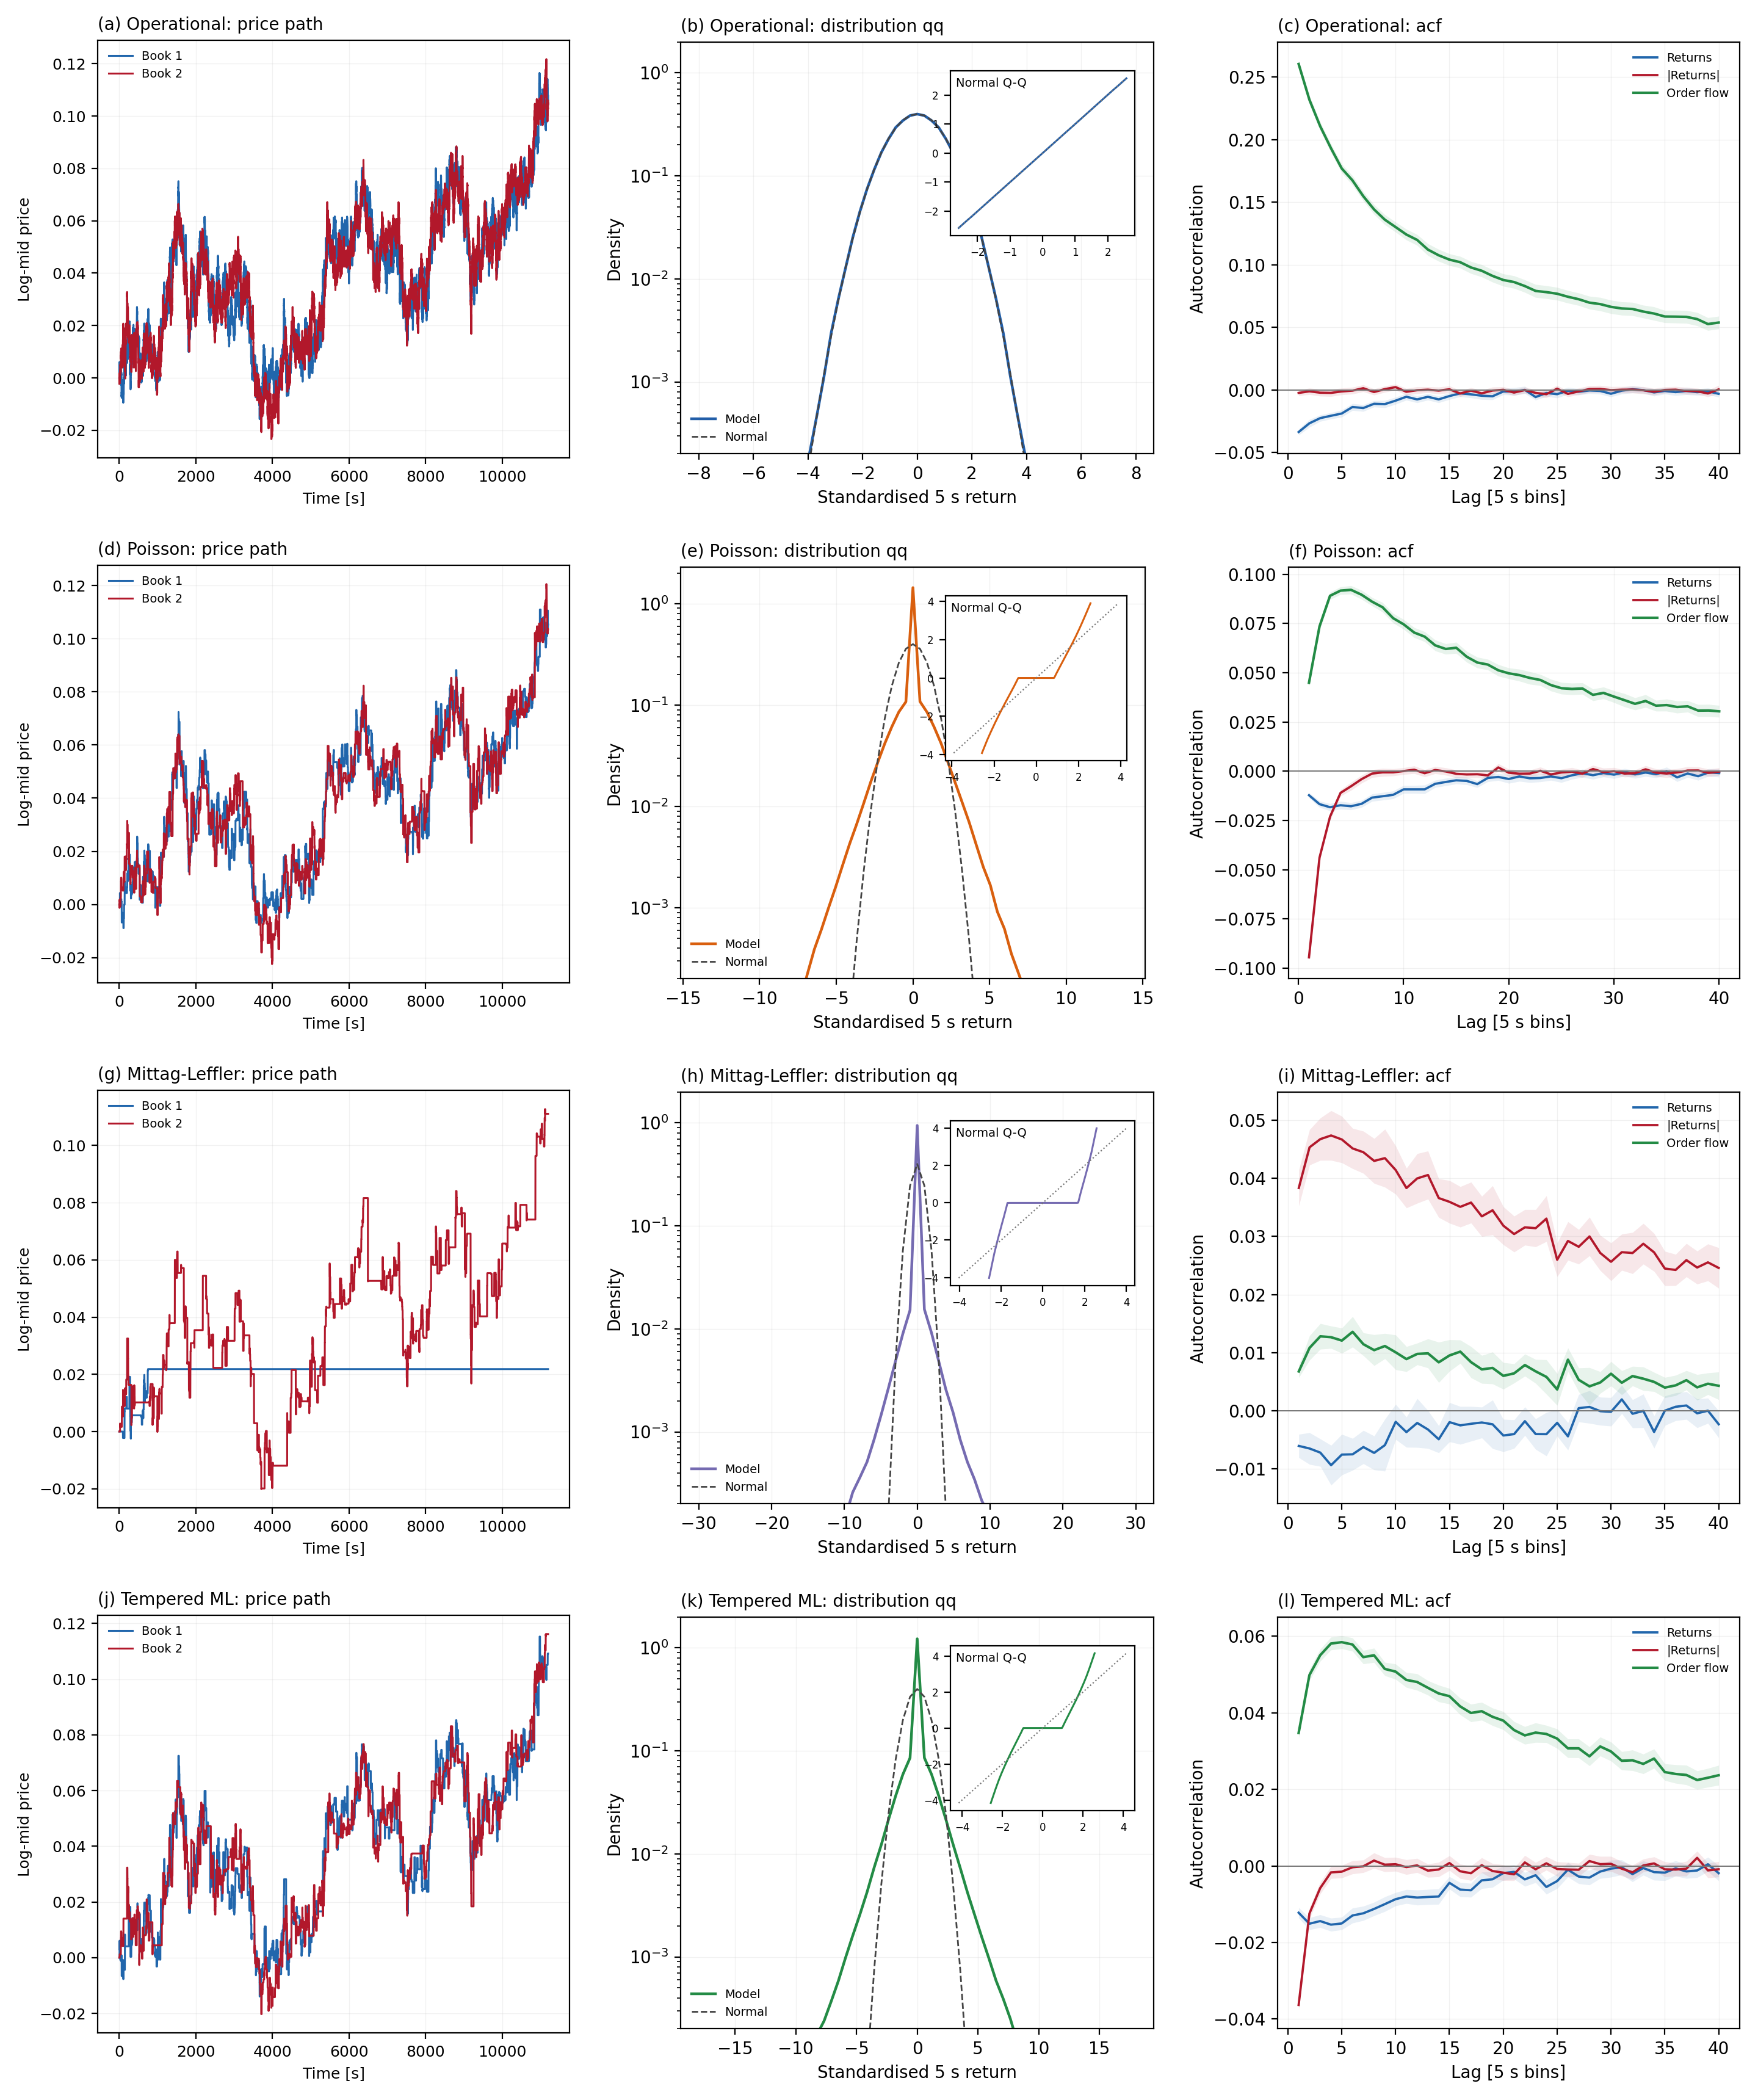
\includegraphics[width=\textwidth]{figures/figure-13-stylised-facts-recovery-v2.png}
\caption{\textbf{Current-model stylised facts under operational and calendar
observation.} Panels (a)--(c) use five-second increments on the uniform
operational grid; panels (d)--(f) use previous-refresh calendar observations
of the same simulated paths. Panels (a) and (d) show the Book 1 log-mid
displacement for the registered representative path, with unstandardised log
returns inset. Panels (b) and (e) show pooled standardised-return densities
with the fixed standard-normal reference and normal-QQ insets. Panels (c) and
(f) show ensemble log-return ACFs, with absolute-log-return and declared-
aggressor signed-order-flow ACFs nested in the same order as Bauer et al. Blue
curves are model estimates; orange is the standard-normal reference, green is
the QQ identity or lower pointwise uncertainty curve, and magenta is the upper
pointwise uncertainty curve. The fixed-grid implementation uses $\alpha_u=1$
and zero cancellation. The calendar path is stepwise because previous-refresh
observation holds the last operational log-mid value between asynchronous
refreshes. This creates a central zero-return mass and stronger calendar-time
tail curvature without changing the underlying operational path. Unlike Bauer
et al. Figure 3, the rows are an operational/calendar comparison rather than
empirical/calibrated data; no empirical row, legacy fractional recurrence or
absolute price-level claim is made. Signed-order-flow persistence is imposed
by the declared finite-persistence input and is not an endogenous result.}
\label{fig:stylised-facts-recovery}
\end{figure}


\clearpage
\begin{landscape}
% Standalone table fragment. Required packages: booktabs, tabularx, array, float.
\begin{table}[H]
\centering
\scriptsize
\caption{\textbf{Parameter, timescale and identifiability register.} The table maps paper notation to implementation names and records units, roles, sensitivity pathways, and fixed or swept status. Refresh rate and source amplitude receive different code names despite source-notation overlap. Identifiability classifications describe the information available from the planned outputs under the stated model; they are not estimates, formal statistical-identifiability proofs, or empirical calibration results.}
\label{tab:parameter-register}
\renewcommand{\arraystretch}{0.98}
\begin{tabularx}{\linewidth}{@{}p{1.7cm}p{3.3cm}p{2.3cm}p{2.5cm}X X X X@{}}
\toprule
Paper symbol & Code name & Source & Units & Role & Sensitivity path & Figure treatment & Identifiability from Epps output \\
\midrule
\(\Delta\) & \texttt{aggregation\_\allowbreak{}scale} & Eqs. (8), (9), (11) & time; dimensionless after scaling & return aggregation horizon & direct horizontal scale & swept in F1-F6 & observed/design variable \\
\(\rho_\infty\) & \texttt{rho\_\allowbreak{}inf} & Eqs. (8), (9), (11) & dimensionless correlation & long-scale vertical level & multiplicative vertical scale & fixed to one in base figures & conditional on plateau coverage \\
\(\lambda_{12}\) & \texttt{clock\_\allowbreak{}rate} & Eq. (8); App. A & time\(^{-1}\) & pooled refresh/overlap rate & \(F(\lambda_{12}\Delta)\) & unit scale; sensitivity in F2 & conditional; independently measurable in v2 \\
\(\kappa=\kappa_1+\kappa_2\) & \texttt{response\_\allowbreak{}rate} & Eq. (9); App. B & time\(^{-1}\) & spread relaxation rate & \(F(\kappa\Delta)\) & swept in F1-F2; derived in F4-F5 & conditional on clock rate and short scales \\
\(\alpha_c\) & \texttt{alpha\_\allowbreak{}clock} & App. C, Eq. (C.18) & dimensionless & fractional clock order & short power \(\Delta^{\alpha_c}\) & swept in F3 & not separate from alpha\_response at short scale \\
\(\alpha_r\) & \texttt{alpha\_\allowbreak{}response} & App. C, Eq. (C.18) & dimensionless & fractional response order & short power \(\Delta^{\alpha_r}\) & swept in F3 & not separate from alpha\_clock at short scale \\
\(\tau_c,\tau_r\) & \texttt{clock\_\allowbreak{}characteristic\_\allowbreak{}time}\newline\texttt{response\_\allowbreak{}characteristic\_\allowbreak{}time} & v1 nondimensionalisation & time & fractional scale convention & \((\Delta/\tau)^\alpha\) & fixed to one in F3 & confounded with fractional rate convention \\
\(\gamma_{jk}\) & \texttt{coupling\_\allowbreak{}strength} & Eq. (6); App. B & model-dependent & pair-trader coupling strength & \(\kappa_j\propto\gamma_{jk}\) & one-at-a-time sweep in F4 & not separate from source/front quantities \\
\(\lambda_j\) (source) & \texttt{source\_\allowbreak{}amplitude} & Eq. (5); App. B & source amplitude & decaying-Gaussian amplitude & \(M_j^+\propto a_j\) & one-at-a-time sweep in F4 & not separate from coupling strength \\
\(\mu_j\) & \texttt{source\_\allowbreak{}width} & Eq. (5); App. B & price\(^{-2}\) & Gaussian source-shape scale & \(M_j^+\propto\mu_j^{-1/2}\) & one-at-a-time sweep in F4 & not separate from amplitude/front slope \\
\(|\mathcal L_j|\) & \texttt{front\_\allowbreak{}slope\_\allowbreak{}abs} & Eq. (B.9); Eq. (B.13) & density per price & frozen reaction-front slope & \(\kappa_j\propto|\mathcal L_j|^{-1}\) & one-at-a-time sweep in F4 & not identifiable as thickness from Epps alone \\
\(\varepsilon\) & \texttt{epsilon} & Eq. (6); App. D & price\(^2\) for \(yz/\varepsilon\) & continuum selector regularisation & centred moment invariant; representation path & swept in F5 & not a reaction-front thickness parameter \\
\(\Delta x\) & \texttt{lattice\_\allowbreak{}spacing} & App. D & price & numerical lattice resolution & discrete moment error to effective response & swept in F5 & known numerical control \\
\(z_{jk}\) & \texttt{directed\_\allowbreak{}spread} & Eq. (6); App. B & price & directed book-price spread & selector argument \(yz/\varepsilon\) & fixed to 0.2 in F5 & state variable, not inferred parameter \\
-- & \texttt{alignment\_\allowbreak{}offset\_\allowbreak{}cells} & v1 numerical diagnostic & lattice cells & source-selector centring error & parity breaking to effective response & 0 and 0.5 in F5 & known numerical control \\
-- & \texttt{domain\_\allowbreak{}halfwidth} & v1 numerical diagnostic & price & finite integration/lattice domain & tail truncation to effective response & full and truncated in F5 & known numerical control \\
\bottomrule
\end{tabularx}
\end{table}

\end{landscape}

\begin{landscape}
% Standalone table fragment. Required packages: booktabs, tabularx, array, float.
\begin{table}[H]
\centering
\scriptsize
\caption{\textbf{Numerical benchmarks, convergence tests and acceptance status.} Each row records a claim-relevant diagnostic, its analytic or independent reference result, declared tolerance, observed value or error, and acceptance status. Checks cover the ordinary kernel and derivative, fractional $\alpha=1$ recovery and independent reference values, the decaying-Gaussian first moment, centred-selector invariance, finite-grid refinement, invalid inputs, and the analytic/simulation overlay contract. The table supports numerical reliability and reproducible execution within the tested environment; it is not a mathematical proof of the model, an empirical validation, or evidence for excluded legacy-simulation claims.}
\label{tab:numerical-benchmarks}
\renewcommand{\arraystretch}{1.02}
\begin{tabularx}{\linewidth}{@{}p{0.9cm}p{3.6cm}X p{3.0cm}X p{1.8cm}@{}}
\toprule
ID & Diagnostic & Expected result & Tolerance & Observed result & Status \\
\midrule
D01 & Ordinary zero and small-argument limit & F(0)=0 and the declared small-x series is recovered & abs error <= 1.0e-12 & F(0)=0.000e+00; series error at 1e-6=0.000e+00 & Verified \\
D02 & Ordinary bounds and monotonicity & 0 <= F(x) < 1 and non-decreasing for x >= 0 & violation <= 1.0e-12 & range=[0.00000500, 0.99000000]; min increment=1.641e-07 & Verified \\
D03 & Ordinary analytic derivative & Analytic derivative agrees with centred finite differences & max error <= 2.0e-07 & max error=2.084e-10 & Verified \\
D04 & Ordinary elasticity limits & S\_F -> 1 at short scale and S\_F -> 0 at long scale & combined limit error <= 2.0e-05 & S(1e-8)=0.999999996667; S(1e5)=1.000e-05 & Verified \\
D05 & Fractional alpha-one recovery & F\_alpha with alpha=1 equals the ordinary kernel & max error <= 2.0e-13 & max error=0.000e+00 & Verified \\
D06 & Fractional independent reference values & Release evaluator matches adaptive-quadrature references & max error <= 2.0e-09 & six-point max error=1.571e-13 & Verified \\
D07 & Fractional bounds and monotonicity & Release curves remain in [0,1] and non-decreasing & violation <= 2.0e-09 & maximum violation=0.000e+00 & Verified \\
D08 & Decaying-Gaussian first moment & Numerical full-domain selected moment equals analytic half-line moment & relative error <= 2.0e-06 & analytic=-0.443113462726; numerical=-0.443113462726 & Verified \\
D09 & Centred-selector continuum invariance & Symmetric first moment is independent of selector width & relative error <= 2.0e-06 & max relative error over three epsilon values=2.220e-16 & Verified \\
D10 & Centred finite-grid convergence & Moment error decreases from a deliberately coarse lattice under refinement & finest error <= 2.0e-05 & errors=1.935e-01,1.939e-03,1.635e-06,1.110e-15 & Verified \\
D11 & Boundary baseline response normalisation & Two-book baseline total response rate equals one & abs error <= 1.0e-12 & kappa\_total=1.000000000000 & Verified \\
D12 & Combined-factor construction & Combined curve equals diagnosed component product and remains bounded & violation <= 1.0e-12 & range=[0.00000025, 0.98010000] & Verified \\
D13 & Invalid-input handling & Four invalid parameter cases fail clearly & all four raise ValueError & caught=4/4 & Verified \\
D14 & v2 analytic/simulation overlay contract & Required scientific and provenance roles are declared & all ten roles present & declared roles=10/10 & Verified \\
\bottomrule
\end{tabularx}
\end{table}

\end{landscape}

\section{Parameter and numerical evidence}

Table~\ref{tab:parameter-register} keeps the source notation, unambiguous code names, units, sensitivity paths, and identifiability qualifications together. In particular, the paper's refresh-rate and source-amplitude uses of \(\lambda\) are separated in code. Table~\ref{tab:numerical-benchmarks} is generated from the diagnostic results; scientific figures are not accepted if a row is failed. The fractional reference points were computed independently with adaptive quadrature, while the release evaluator uses fixed composite Gauss--Legendre quadrature and a small-argument series.

\section{Reproducibility contract}

The complete active route is
\begin{verbatim}
python scripts/run_all.py
\end{verbatim}
and the standard-library regression tests are
\begin{verbatim}
python -m unittest discover -s tests -v
\end{verbatim}
The run regenerates or scientifically verifies the thirteen selected PDF/PNG figure pairs, two CSV/LaTeX table pairs, claim-bearing curve and summary datasets, diagnostic reports, and the retained simulation route. PDF bytes can differ across systems because of renderer metadata or font embedding; frozen inputs, machine-readable values, declared tolerances and diagnostic statuses are the cross-platform reproducibility objects.

The accepted analytical output schemas retain their scientific object versions. The final simulation evidence is registered in the component, combined, impact and dependence CSV files listed in the figure manifest. Simulation resolution, alignment and domain metadata accompany the comparisons because Figure~\ref{fig:grid} shows that numerical boundary representation can move the apparent response curve.

\section{Interpretive limits}

The diagnosed computations support a limited set of conclusions. Ordinary clock and coupling factors are distinguishable when their timescales are sufficiently separated and the components are shown explicitly. The long-scale plateau contains little local information about either rate. The leading short-scale power of a combined fractional curve identifies an order sum rather than two separate orders. Reaction-boundary quantities affect the Epps curve conditionally through the effective response rate, but are not individually identified by that curve. Continuum selector invariance can coexist with finite-grid distortion when parity, alignment or domain controls are not respected. The translation-mode simulation is consistent with the registered component curves and improves the no-refit combined comparison when the estimator's finite-grid, finite-step clock selection is represented exactly. The impact, shock-recovery, autocorrelation and stylised-facts figures are conditional model diagnostics, not empirical calibration.

These are computational illustrations and numerical verification statements inside the paper's assumptions. They are not empirical validation, calibration or proof of the approximations. The retired Bauer implementation is not required to execute or interpret the accepted v2 route.

\medskip
\noindent\textbf{Software and licensing note.} Code is provided under the MIT License; supplementary text, captions, generated figures, tables, and documentation are provided under CC BY 4.0. The paper and frozen source retain their existing terms.

\end{document}
